\documentclass[11pt, a4paper]{report}

% Page styling
\usepackage{extsizes}
\usepackage{latexsym}
\usepackage[a4paper,margin=3cm]{geometry}
\usepackage{changepage}

% Spacing
\usepackage{setspace}

% Tables
\usepackage{tabularx,ragged2e}
\usepackage{booktabs}
\setlength{\columnsep}{1cm}

% Links
\usepackage{hyperref}

% Lists
\usepackage{enumitem}

% Figures
\usepackage{float}
\usepackage{subfig}
\usepackage{caption}
\captionsetup[figure]{font=small,labelfont=Small}

% Equations% Equations & Theorems
\usepackage{amssymb}
\usepackage{amsmath}
\usepackage{amsthm}
\usepackage{amsfonts}
\usepackage{thmtools}
\usepackage{graphicx,color}

% Citations
\usepackage{biblatex}
\addbibresource{citations.bib}



%----------------------------------------------------------------------------------
% Title Page
%----------------------------------------------------------------------------------
\title{{\vspace{-2in}
\includegraphics[width=\textwidth]{docs/Project Report/Media/ucl_logo.png}}\\
\vspace{2cm}
\begin{adjustwidth}{1cm}{1cm}
    \centering
    \Huge Robust Robotic Grasping Utilising Touch Sensing
\end{adjustwidth}}
\\
\date{Submission date: \today}
\author{COMP0029\_ZZJN7\thanks{
{\bf Disclaimer:}
This report is submitted as part requirement for the BSc degree in Computer Science at UCL. It is
substantially the result of my own work except where explicitly indicated in the text.
\emph{Either:} The report may be freely copied and distributed provided the source is explicitly acknowledged
\newline
\emph{Or:}\newline
The report will be distributed to the internal and external examiners, but thereafter may not be copied or distributed except with permission from the author.}
\\ \\
BSc Computer Science\\ \\
Supervisors: Prof. Marc Deisenroth, Dr. Yasemin Bekiroglu}



\begin{document}
\onehalfspacing
\maketitle
\pagenumbering{roman}

%----------------------------------------------------------------------------------
% Abstract
%----------------------------------------------------------------------------------
\begin{abstract}
Robotic grasp synthesis has been studied extensively as robotic grasping skills have a significant impact on the success of subsequent manipulation tasks. Various approaches have been proposed for robotic grasp planning, with different assumptions regarding the available information about the type of objects in question (known, unknown, familiar). These approaches range from heuristic rules, and designing simplifying hand models, to complete end-to-end systems inferring grasp parameters from raw data.\\

However, most of these approaches do not address robustness in grasping, which refers to the ability of a robot to perform a grasping task consistently and accurately even in the case of unexpected disturbances or large degrees of errors in perception. There are several fundamental problems that need to be addressed to achieve better robustness in grasping tasks. These include mainly dealing with uncertainties in sensing, actuation and perceptual data.\\

In this project, we study how to build a robust learning framework that can be employed to construct robust grasp configurations using multi-modal data, e.g. tactile, and visual. The project addresses the following main issues with the robotic grasping systems: a) balancing the trade-off between data representation and data dimensionality; b) analysing the modelling effects of different modalities, e.g. tactile and visual, and features to capture the underlying characteristics of the overall grasping process; c) a correction policy that relies on assessing grasp success before further manipulation using perceptual data, to choose the right grasping configuration.
\end{abstract}


%----------------------------------------------------------------------------------
% Acknowledgements
%----------------------------------------------------------------------------------
\renewcommand\abstractname{Acknowledgements}
\begin{abstract}
    
\end{abstract}


%----------------------------------------------------------------------------------
% Contents
%----------------------------------------------------------------------------------
\tableofcontents


%----------------------------------------------------------------------------------
% Chapter 1: Introduction
%----------------------------------------------------------------------------------
\chapter{Introduction}
\label{chap:1}
\pagenumbering{arabic}
\setcounter{page}{1}


\section{Motivation}
\label{sec:1.1}
Humans are able to grasp objects seemingly intuitively. We can efficiently identify and reach for objects, adjust our finger placements and optimally balance contact forces by coordinating our wrists, arms, and shoulders when we approach and lift objects. Our sense of touch plays a major role, providing us with information about the object's size, shape, texture, weight, and other physical properties. This information is processed by sensorimotor and cognitive functions \cite{castiello2005} in our brains, giving us instructions on how to adjust our grasp pose and apply the appropriate amount of force needed to pick up the object. Without the sense of touch, grasping objects would be much more difficult and less efficient.\\

For several decades, researchers have delved into the domain of robotic grasping to equip real-life robots with the ability to grasp objects. Various techniques have been introduced in this field, such as the incorporation of touch sensing \cite{de_Farias_2021} using tactile sensors \cite{Lambeta2020DIGIT, liu2022gelsight} and/or visual perception \cite{Calandra_2018}. These methods enable robots to determine grasp configurations that meet a set of criteria that are relevant to the grasping task, which is known as grasp synthesis \cite{Bohg_2014}. However, obtaining appropriate grasp configurations has proven to be a challenging task since it requires identifying an infinite set of grasp candidates given a $n$-dimensional pose of a robotic arm and gripper joints, where $n$ is the number of movable joints. Thus, most approaches to grasp synthesis are categorised into two main groups \cite{Bohg_2014, SAHBANI2012326}: analytical and data-driven methods. Analytical methods treat grasp synthesis as constrained optimisation problems that measure dexterous, stable, and dynamic behaviour properties using heuristics. In contrast, data-driven methods rely on sampling grasp candidates for an object and ranking them based on a pre-determined metric \cite{Bohg_2014}.\\

In recent years, the combination of physical simulators and machine learning has led to significant advancements in the field of robotic grasping. One of the key challenges in robotic grasping is developing algorithms that can handle the complexity and variability of the real world. Physical simulators such as Pybullet \cite{coumans2021} provide a valuable tool for generating large amounts of training data, allowing machine learning algorithms to learn from simulated experiences before being deployed on physical robots with minimal additional tuning \cite{berscheid2020selfsupervised}. Researchers have also utilised physical simulators to train robotic grasping policies \cite{Chebotar_2017} and transfer them to the real world, and have proven that data-driven approaches outperform classical methods \cite{zhang2022robotic}.
\begin{figure}[ht]
    \centering
    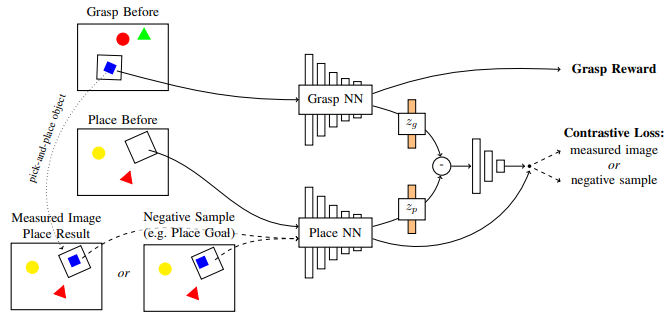
\includegraphics[width=\textwidth]{docs/Project Report/Media/1_1_berscheid_2020_sl_for_precise_pickandplace_wo_obj_model_network.png}
    \caption{Berscheid et al.: Self-supervised learning for Precise Pick-and-place without Object Model \cite{berscheid2020selfsupervised}: A purely data-driven approach to generating data for self-supervised learning for robotic grasping using neural networks and object recognition}
    \label{fig:1.1}
\end{figure}

However, little work has been done on increasing robustness in grasping systems that utilise multi-modal (tactile and visual) data. Robustness in robotic grasping is a crucial property for ensuring effective and reliable manipulation of objects in a wide range of scenarios. It refers to the ability of a robotic grasping system to perform successful grasps despite uncertainties and variations in the environment and object properties (geometric, physical). One of the primary challenges in robotic grasping is the wide variety of shapes and sizes that objects can come in. This can make it difficult for a robotic grasping system to determine the best approach for grasping, as well as to adjust its grasp strategy based on the object's properties. A robust system should be able to handle these variations and adjust its grasp strategy accordingly to ensure that the object is firmly held during manipulation. Another challenge is posed by uncertainties in the object's pose. Objects can be placed in various orientations and positions, making it challenging for a robot to determine the optimal grasping location. A robust system should be able to estimate the object's pose accurately and choose an appropriate grasp location to ensure that the object is grasped correctly. Furthermore, the environment in which a robot operates can change unpredictably, with variations in lighting conditions, surface textures, and other factors affecting the ability of a robotic grasping system to perform well. A robust system should be able to adapt to these changes and adjust its grasping strategy accordingly.\\


We aim to take the best of both analytic (24) and data-driven methods \cite{berscheid2020selfsupervised, pinto2015supersizing} to develop robust and scalable grasping methods. Robustness in a robotic grasping system refers to its versatility of accurately recognising and grasping objects with varying geometric features (width, depth, curvature, etc) and its ability to successfully grasp the objects. Robustness is increasingly becoming a vital factor in the study of grasp stability and quality, however, incorporating robustness makes it practically difficult to design a single gripper that can effectively grasp all objects. As a result, researchers and engineers have developed dedicated grippers tailored to specific grasping tasks or types of objects.\\

However, developing a robust and efficient grasping system presents several challenges. One major hurdle is the incorporation of touch sensing into robotic grasping, which is hindered by hardware limitations such as sensor sensitivity and cost, as well as difficulties in integrating tactile inputs into standard control schemes \cite{Calandra_2018}. Consequently, most robotic grasping research has focused on vision and depth as the primary input modalities \cite{Calandra_2018, de_Farias_2021}.
\begin{figure}[ht]
    \centering
    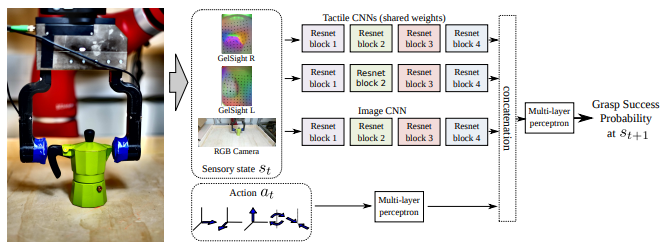
\includegraphics[width=\textwidth]{docs/Project Report/Media/1_1_calandra_2018_model.png}
    \caption{Calandra et al.: More Than a Feeling: Learning to Grasp and Regrasp using Vision and Touch \cite{Calandra_2018}: A study on learning regrasping policies from multi-modal (tactile and visual) data by predicting the grasp stability outcome of a candidate grasp adjustment, then executing a grasp by iteratively selecting the most promising actions}
    \label{fig:1.2}
\end{figure}

However, vision-based grasping approaches have limitations in measuring and reacting to ongoing contact forces, which hinders the full potential benefits of interaction. As a result, these approaches mostly rely on pre-selecting a grasp configuration, such as location, orientation, and forces, before making contact with the object. Addressing these limitations and integrating tactile feedback could significantly improve robotic grasping, leading to more efficient and effective interactions between robots and the physical world.\\

Another challenge is developing a concrete strategy for improving grasp quality and planning while conserving the efficiency of the overall system. Such strategies can be summarised into three types: (1) choice of object representation, where coarse approximations of the underlying true shape of an object can simplify the generation of new grasps \cite{de_Farias_2021} \cite{geidenstam_2009}; (2) use of local symmetry properties to capture key geometric features of the object to generate promising grasp candidates \cite{de_Farias_2021}; (3) optimising shape modelling where target objects are parameterised using smooth, differentiable functions from point clouds using spectral analysis \cite{de_Farias_2021}.


\section{Project Aims}
\label{sec:1.2}
Having gained a comprehensive understanding of the previously discussed optimisations and strategies, our research project focuses on the development and testing of a robust robotic system that can learn to pick up an object with simple geometry using a two-finger hand. The project will take a learning-based approach to grasping through, for example, Bayesian optimisation \cite{nogueira2016unscented, frazier2018tutorial}. The learning-based approach should be compared with a baseline approach from the related literature (e.g. \cite{nogueira2016unscented, danielczuk2020exploratory, breyer2020volumetric}) for evaluation, for example, a simple regression classifier to differentiate between good and bad grasps.


\section{Project Objectives}
\label{sec:1.3}
This project is concerned with the development of a complete simulation with supporting features for data collection and analysis. Therefore, the aims of this project are split according to our system requirements, which we describe in detail below. These objectives are expected to be completed throughout the academic year:
\begin{enumerate}
    \item Set up a simulation environment, e.g. PyBullet \cite{coumans2021} or NVIDIA Isaac. 
    \item Create a data collection pipeline for sensory data (e.g. visual and force/torque readings) via the simulator.
    \item Apply basic simulation functionalities: position control and vision sensing on the robot.
    \item Implement and test baseline (e.g. \cite{breyer2020volumetric}, and a basic approach such as executing predefined grasps per object model given object pose).
    \item Build the learning framework:
    \begin{enumerate}
        \item Learning grasps based on Bayesian Optimisation, from a chosen scene representations such as signed distance function 
        \item Picking with two fingers given object model (primitive shapes such as box, sphere, cylinder) and pose, all learned by trial and error
    \end{enumerate}
\end{enumerate}


\section{Project Approach}
\label{sec:1.4}
This section discusses the important phases of the project and the approach taken at each phase. Technologies required for completing a particular phase will be documented and justified.


\subsection{Planning Phase - Design and Research}
\label{sec:1.4.1}
We first conduct a literature survey to explore and categorise research projects related to robotic grasping by data input, grasping method and the problem these projects address. Simultaneously, background research was conducted on grasp learning \cite{platt2022grasp} and robot manipulation to obtain a general understanding of the project's task.


\subsection{Early Development Phase - Pybullet Simulation}
\label{sec:1.4.2}
This project is completely conducted via a simulation environment, including data collection, robot manipulation, experimentation and testing of our approaches. Therefore, the development of a Pybullet simulation was considered a top priority in the early phases of the project. The robot we used for our simulation consists of the following components:
\begin{enumerate}
    \item Arm: UR5 Robot Arm Manipulator
    \item Gripper: Robotiq 2-Finger Adaptive Robot Gripper 85
    \item Tactile sensors: DIGIT tactile sensors \cite{Lambeta2020DIGIT} mounted onto each finger of the gripper
\end{enumerate}
The Pybullet simulation should support the following features for our project:
\begin{enumerate}
    \item manual robot (end effector) manipulation
    \item real-time display of tactile data (depth and colour cameras)
    \item a grasp planner using inverse kinematics
    \item a random end effector pose generator for creating varying grasp poses
    \item a tactile data collection pipeline using randomly-generated end effector grasp poses
\end{enumerate}
\noindent This will be further discussed in \hyperref[sec:3.1]{Section 3.1}.


\subsection{Baseline Development Phase}
\label{sec:1.4.3}
This phase focuses on determining the optimal dataset representation for our collected multi-modal data, consisting of tactile sensor readings, visual end effector poses relative to the arm, and the respective grasp outcomes of each end effector pose. In addition, we experiment with several feature engineering techniques, for example, dimensionality reduction using ConvNets and Principal Component Analysis (PCA).


\subsection{Execution Phase - Learning Approach Implementation}
\label{sec:1.4.4}
Following the outcomes of our baseline approach where we identified the optimal feature representation of our dataset, we move on to develop our learning-based approach which is trained on three primitive object types. In addition to tactile sensor readings and visual data (randomly-generated end effector poses), we include the object features for each object class in our dataset, and train this dataset on a multi-layer perceptron (MLP). Finally, we conduct several interesting experiments, including (1) training our MLP using various dataset segmentations; and (2) validating our MLP on unseen objects that comprise similar geometric features to that of the primitive objects that our MLP was trained on.


\subsection{Documentation Phase}
\label{sec:1.4.5}
The final phase of the project involves the completion of the project report, writing documentation on setting up and using the simulation, as well as including a brief description of the methodology behind our baseline and learning-based approaches which are implemented in Jupyter Notebook.


\section{Report Structure}
\label{sec:1.5}
Chapter 2 gives a brief overview of the background of robotic grasping and relevant literature on the project. We investigate common grasp representations and grasp quality evaluation techniques, and analyse various data representations of multi-modal data (tactile, sensory, temporal) and policy-learning approaches.\\

Chapter 3 documents the system architecture for the project and the development of a Pybullet simulation, including input components to enable data collection and simulation of our robot setup.\\

Chapter 4 documents the development and testing of our baseline approach using a binary logistic regression classifier.\\

Chapter 5 documents the development and testing of our proposed approach using a multi-layer perceptron (MLP) model that attempts to infer good grasp configurations on three primitive object classes from random hand poses, trained on data collected from the Pybullet simulation. The dataset includes tactile sensor readings, random hand poses and geometric features of the target objects.\\

Chapter 6 summarises the results and performances of the project, as well as makes suggestions for future work and improvement based on these findings.



%----------------------------------------------------------------------------------
% Section 2: Background and Literature Review
%----------------------------------------------------------------------------------
\chapter{Background and Literature Review}
\label{chap:2}


\section{Robotic Grasping}
\label{sec:2.1}
In the field of robotics, grasping is a fundamental yet challenging skill of robots which refers to the autonomous ability of a robot to grasp and move objects with its mechanical grippers or other end effectors \cite{zhang2022robotic}. It demands precise coordination between the visual perception of the surrounding environment and efficient grasp planning, as well as a robot's adaptiveness to unseen object classes (robustness).\\

Robotic grasping is far away from developing into an intuitive and instinctive sense as in human beings. There are many unknown factors that enable humans to flawlessly perform grasps when provided with visual and tactile information. However, with the advancements of deep learning and computer vision, semantic grasping is becoming the main focus and basis for autonomous robotic grasping systems \cite{zhang2022robotic}, where a robot is trained on monocular images of a user-specified object type \cite{jang2017endtoend}.\\

To successfully grasp an object, a robot needs to detect the object's location (through, for example, a wrist camera), orientation, and size accurately, estimate the best grasp point and orientation, and then execute the grasp with appropriate force and control to ensure a secure hold. The grasping process can be performed using various types of end effectors, including grippers, suction cups, or specialised tools designed for specific tasks.\\

Therefore, accurate and efficient grasp representation and planning are paramount to ensure a smooth grasping process when performing grasping tasks.


\newpage
\subsection{Grasp Representation}
\label{sec:2.1.1}
A grasp in robotic grasping is a specific configuration of a robotic hand or gripper which allows it to firmly hold an object. These representations can be used in different grasp planning algorithms and can be combined to create more complex representations of grasps. Commonly-used grasp representations include: 


\subsubsection{Meshes}
\label{sec:2.1.1.1}
In computer graphics and object modelling, a (polygon) mesh is a 3-dimensional representation or rigid reconstruction of the surface of an object. Typically, the representation is a collection of vertices, edges and faces that define the object's shape. Faces usually consist of triangles an object's surface that is composed of vertices, edges, and faces. Grasps can be represented as a set of vertices on the mesh that corresponds to the location of the gripper's fingertips and palm.


\subsubsection{Point Clouds}
\label{sec:2.1.1.2}
In the context of robotics, a point cloud is a discrete set of 3-dimensional Cartesian coordinates which collectively represents the surface of an object. The location of a gripper's fingertips can be represented as sets of points on the point cloud in order to annotate a grasp.\\

In addition to grasp representations, point clouds can be merged for surface reconstruction (using, for example, Poisson surface reconstruction), which creates a mesh (or set of surfaces) that approximate the true shape of the target object.\\

In the Pybullet simulation for this project, we include a simple feature that generates a point cloud of the rendered object of the simulation which can be inspected visually. In the physical world, a point cloud is generated using 3D scanners or photogrammetry software, which can be rendered and inspected in a virtual world.


\subsubsection{Hand Configurations}
\label{sec:2.1.1.3}
A hand (or end effector) configuration describes the joint angles or positions of a robotic hand or gripper relative to the robot itself. This is a simple and straightforward approach to representing grasps.\\

In this project, we use the terms "hand configurations" and "end effector poses" interchangeably.


\section{Tactile Sensing for Robotic Grasping}
\label{sec:2.2}
Tactile sensing has been widely used to provide robots with information about target objects, allowing them to grasp and manipulate said objects with greater precision.

\begin{enumerate}
    \item detect object properties
    \item monitor grasp stability (Yasemin's thesis)
    \item provide feedback during manipulation, detect object contact
\end{enumerate}


\section{Common Grasping Approaches}
\label{sec:2.3}
Humans rely on rich tactile feedback to grasp objects, however, most of the recent robotic grasping studies only focus on visual input. The authors propose an end-to-end action-conditional model (a multimodal CNN) to learn regrasping policies from visual-tactile data, by predicting the outcome of a candidate grasp adjustment, then executing a grasp by iteratively selecting the most promising actions\cite{Calandra_2018}.


\section{Conclusion}
\label{sec:2.4}
Conclude that not much work has been done on using tactile + visual data for robust grasping systems



%----------------------------------------------------------------------------------
% Section 3: Preliminaries
%----------------------------------------------------------------------------------
\chapter{Preliminaries}
\label{chap:3}
In this chapter, we present the practical aspects of the project. We first provide an overview of the Pybullet simulation and its functionalities specific to the project.


\section{Pybullet Simulation Overview and Functionalities}\label{sec:3.1}
Pybullet is a Python module designed for robotics simulation and machine learning purposes, specifically emphasising sim-to-real transfer, as indicated by Coumans and Bai \cite{coumans2021}. In this project, Pybullet's functionalities play a crucial role, such as:
\begin{enumerate}[\itemsep=0em]
    \item Allows the loading of articulated bodies from a variety of file formats, such as Universal Robot Description Files (URDFs), enabling the development of complex robotic systems;
    \begin{figure}[H]
        \centering
        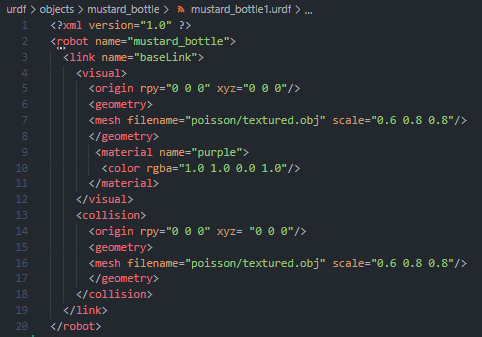
\includegraphics[width=0.6\textwidth]{docs/Project Report/Media/3_1_urdf_eg.png}
        \caption{Example of a URDF file that describes a bottle}
        \label{fig:3.1}
    \end{figure}
    \vspace{-0.2cm}
    \item Provides forward dynamics simulation and inverse dynamics computation, enabling accurate physical modelling of robot movements and interactions with the environment;
    \item Offers collision detection queries, which play a vital role in robot safety and efficiency.
\end{enumerate}
A system architecture diagram for our Pybullet simulation can be found in the \hyperref[]{Appendix}.


\subsection{Role of the Pybullet Simulation}\label{sec:3.1.1}
In the scope of this project, the Pybullet simulation plays a fundamental role in the acquisition of both visual and tactile data. By simulating the robot's dynamics and its interactions with the environment, Pybullet generates data that can be exploited for the purpose of training machine learning algorithms or assessing control strategies. Furthermore, the collected data may also be utilised for analytical purposes, such as the evaluation of the efficacy of distinct robotic designs or the appraisal of the performance of a specific algorithm. Figure 3.1 is a screenshot of our Pybullet simulation with core user-defined parameters on the right panel. Some important parameters include:
\begin{enumerate}
    \item Manually manipulate of the end effector position of the robot gripper (via the sliders)
    \item Data collection pipelines for the baseline and proposed approaches (via the \verb|Collect Data| buttons)
\end{enumerate}

\begin{figure}[H]
    \centering
    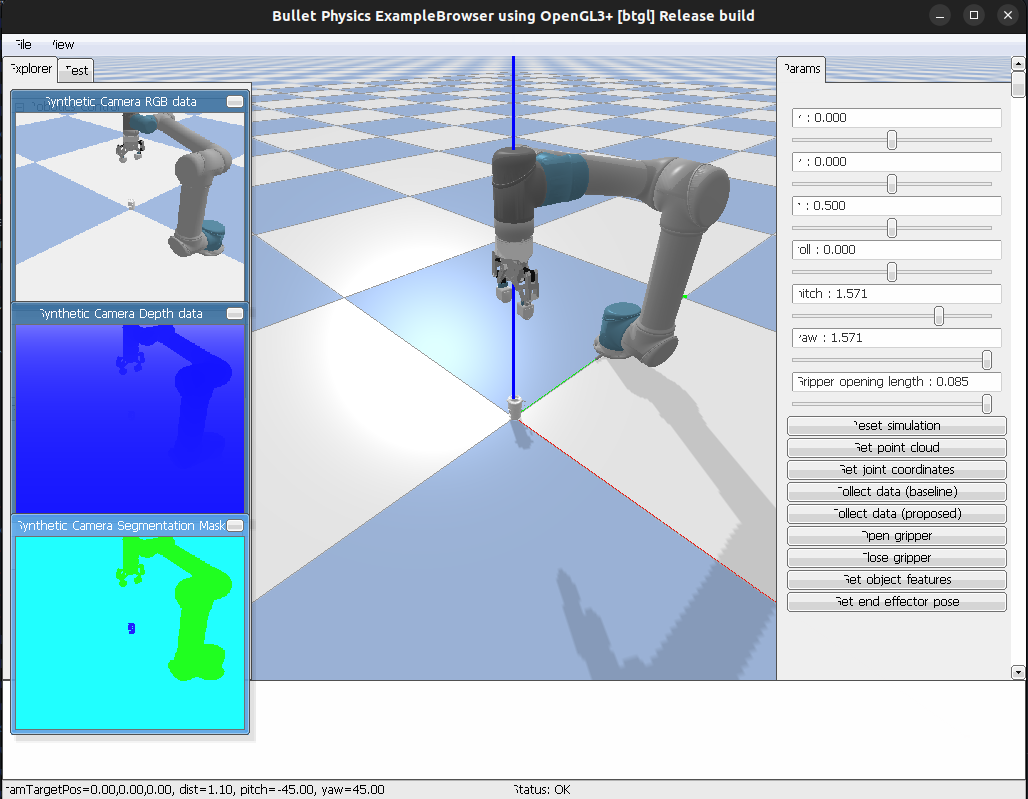
\includegraphics[width=\textwidth]{docs/Project Report/Media/3_1_1_pybullet_sim.png}
    \caption{A screenshot of the Pybullet simulation for this project. The left panel displays real-time visualisations of colour (RGB) and depth data. The right panel includes parameters that can be manually controlled to manipulate the robot setup to perform specific tasks.}
    \label{fig:3.2}
\end{figure}


\subsection{Loading Parameters}\label{sec:3.1.2}
This project allows users to configure the simulation via pre-defined parameters, including Pybullet camera positions and orientations, object variations, and robot setup parameters (e.g., Cartesian position, speed of grippers, etc.), by loading them through the \verb|parameters.yaml| file. YAML is a widely-used format for configuration files that is both human-readable and machine-parsable. In a YAML file, data is structured in a hierarchical system of key-value pairs, which are expressed in a plain-text format.
\begin{figure}[H]
    \centering
    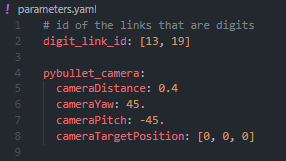
\includegraphics[width=0.5\textwidth]{docs/Project Report/Media/3_1_2_yaml.png}
    \caption{Snippet of the {\verb|parameters.yaml|} configuration file for the Pybullet simulation}
    \label{fig:3.3}
\end{figure}


\subsection{Robot Control and Data Collection}\label{sec:3.1.3}
Our Pybullet simulation consists of two data collection pipelines for the baseline and proposed approaches respectively (see \hyperref[sec:4.2.2]{Section 4.2.2}). These pipelines are activated through the \verb|Collect Data| buttons on the right panel in the simulation. The data collection pipelines randomly generate end effector poses around the vicinity of the target object. Every time a new pose is generated, the robot's position and orientation are reset, and we move the robot to the generated pose via inverse kinematics provided by Pybullet.



\section{Description of Data}\label{sec:3.2}
This work employs the terms "tactile" and "visual" data with frequent recurrence. A comprehensive elucidation of these terminologies shall be presented in the forthcoming sections. To acquire the majority of the data, we utilise "cameras", which are devices that capture sensory data by means of imaging objects being grasped as well as their surrounding environment. In the domain of robotic grasping, cameras are typically installed on a robot gripper and are capable of capturing diverse image types contingent on the given task. In \hyperref[sec:3.2.4]{Section 3.2.4}, we shall delve further into how the real-time visualisation of depth and colour image representations of tactile data is achieved within our simulation.


\newpage
\subsection{Tactile data}\label{sec:3.2.1}
In robotic grasping, tactile data refers to rich information collected from contact with a robotic hand or gripper during the manipulation of objects. It reflects the amount of force and pressure applied by the gripper on an object in the grasping process. Tactile data can be extracted from tactile sensors (cameras) mounted into robotic end effectors or grippers, which can be used to provide feedback to the control system about the grasp quality, such as whether the object is slipping or not, and to adjust the gripper's position and force to improve the grasp. In our simulation, we mount DIGIT tactile sensors \cite{Lambeta2020DIGIT} to each finger of a 2-finger gripper, thus generating a pair of tactile (depth and colour) readings per finger.
\begin{figure}[H]
    \centering
    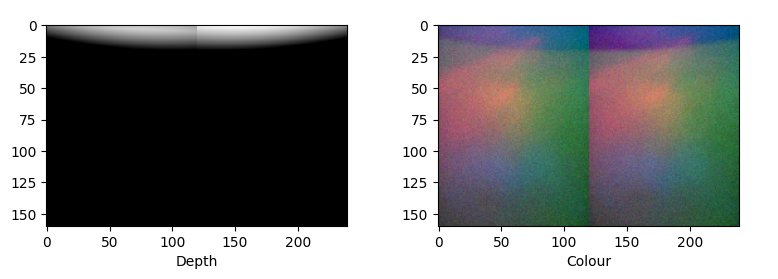
\includegraphics[width=\textwidth]{docs/Project Report/Media/4_2_tactile_data_visualisation.png}
    \caption{Example pair of depth and colour images extracted from the DIGIT cameras}
    \label{fig:3.4}
\end{figure}


\subsection{Visual data}\label{sec:3.2.2}
Visual sensing is an intuitive way for a robot to perceive its environment and is widely used in robotic grasping \cite{GUO2017274}. In this work, visual data refers to information collected by cameras in our simulation. Our visual data will consist of any of the following data sources:
\begin{enumerate}
    \item 6-Dimensional end effector poses relative to the robotic arm/gripper. We refer readers to \hyperref[sec:4.2.1]{Section 4.2.1} for a detailed description of this data.
    \item Geometric features of target objects, which we utilise in \hyperref[chap:5]{Chapter 5}
\end{enumerate}


\subsection{DIGIT Camera for Live Tactile Data Visualisation}\label{sec:3.2.3}
The PyBullet simulation visualisation tool is based on OpenGL and provides a 3D rendering of the simulated environment. Users can manipulate the camera view, zoom in and out, and move around the simulation environment using the mouse and keyboard. The GUI also provides tools for controlling the simulation, such as pausing and resetting, and for editing the simulated objects.\\

In addition to the basic visualisation capabilities, the PyBullet GUI also supports advanced features such as rendering depth and segmentation maps, displaying sensor data from cameras and other sensors, and recording and playing back simulations. It also provides a Python scripting interface that allows users to automate tasks and customise the visualisation and simulation behaviour.\\

DIGIT cameras in PyBullet \cite{Wang2022TACTO} are often used in conjunction with the "Camera Sensor" feature, which allows users to specify the position, orientation, and other parameters of a virtual camera within a simulated environment. Once configured, the camera can be used to capture RGB images, depth maps, or other types of sensor data from the environment. The captured images can then be used as input to machine learning models, or as visual feedback for controlling robotic agents within the simulation.

\begin{figure}[H]%
    \centering
    \subfloat[\centering Real-time colour and depth readings from DIGIT camera]{{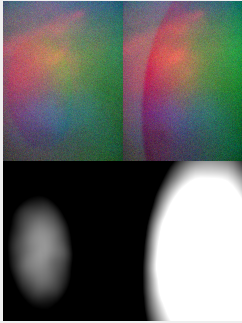
\includegraphics[width=0.41\textwidth]{docs/Project Report/Media/3_2_4_digit_camera.png}\label{fig:3.5a}}}%
    \qquad
    \subfloat[\centering Pybullet robot gripper and object state]{{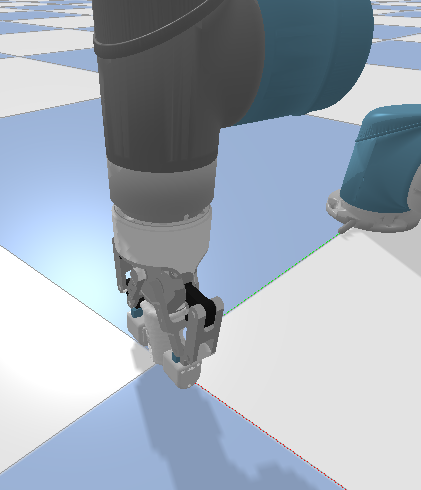
\includegraphics[width=0.47\textwidth]{docs/Project Report/Media/3_2_4_pybullet_arm.png}\label{fig:3.5b}}}%
    \caption{Demonstration of real-time visualisation of tactile sensory readings via DIGIT tactile sensors with Pybullet}%
    \label{fig:3.5}%
\end{figure}

To generate live visualisations of colour and depth sensory data, we configure the DIGIT camera sensor within our Pybullet simulation by specifying its position and orientation relative to the sensors. Next, we capture the sensor data from the simulation and feed it into the DIGIT camera sensor, and finally use Pybullet's built-in visualisation tool which provides real-time visualisation of Pybullet physics simulations to display live visualisations of the tactile sensor data.



%----------------------------------------------------------------------------------
% Section 4: Learning Feature Representations
%----------------------------------------------------------------------------------
\chapter{Learning Feature Representations}
\label{chap:4}
This chapter introduces a baseline approach to grasp stability prediction using a binary logistic regression model. In a previous study conducted by Alkhatib et al. \cite{9091340}, a regularised logistic regression model was used to determine the robustness and quality of grasps and predict their stability. The model's inputs were derived from a set of features measured at each joint of a robotic hand, which were subsequently utilised for training the logistic regression model. In our approach, we use tactile and visual data instead of joint data to classify binary grasp stability labels.\\

In addition, we address a pressing issue of the project - high dimensionality data collected from our simulations. In the previous chapter, we highlighted that a significant portion of the data collected from our simulation is high-dimensional. High-dimensional data poses a significant challenge in terms of computational processing and feature identification. The risk of overfitting also increases as the dimensionality of the data grows, leading to sub-optimal performance of the grasping policy. To mitigate these challenges and effectively train the grasping policy, it is imperative to reduce the data's dimensionality and represent it more concisely.\\

Dimensionality reduction and feature representation techniques can be employed to reduce the data's dimensionality and represent it in a more meaningful way. By doing so, we can identify the most relevant features for the grasping task and reduce the risk of overfitting. Techniques such as Principal Component Analysis (PCA) can be used to determine the most important features in the data. Alternatively, Convolutional Neural Networks (CNNs) can automatically learn features from images or depth maps. A previous study \cite{Calandra_2018} has demonstrated the effectiveness of CNNs in extracting features from high-dimensional data for grasping tasks.\\

To determine an appropriate feature representation, we adopt a binary logistic regression model (commonly known as binary logit) for the classification of grasps and evaluation of the accuracy of the model on various feature representations. Logistic regression is a widely used binary classification algorithm that can be effectively applied to datasets with non-linear relationships, as may exist between the multi-modal features and grasp stability label in our project. It serves as a strong baseline for our investigation, as it provides interpretable results that facilitate the understanding of the effectiveness of the chosen feature representations.\\


\section{Logit Model for Grasp Classification}\label{sec:4.1}
The fundamental assumption of this approach is that grasps can be classified as either successful or unsuccessful outcomes.  In this study, we classify successful hand configurations as those that result in a stable grasp of the object in question. However, there are more sophisticated methods for categorising grasps, which we refer the reader to \cite{Bekiroglu2012LearningTA, si2022grasp}.\\

Assume that we have selected some representation of tactile and/or visual features for each grasp candidate, denoted $x_i$. Our logit model attempts to classify the grasp with a binary label $y_i$. To achieve this, the weights $w$ of the model are fitted through a maximum likelihood estimation where the distribution of the features $x_i$ sits. Assuming the grasp outcomes as a Bernoulli random variable, we can construct and minimise the following cross-entropy loss function and treat it as an optimisation problem:
\begin{equation}
    \ln(L(w))=\sum^n_{i=1}y_i\cdot ln(\rho_y(y_i=1|x_i))+(1-y_i)\cdot\ln(\rho_y(y_i=0|x_i))
\end{equation}
where $\rho_y(y_i=1|x_i)$ and $\rho_y(y_0=1|x_i)$ represent the probability of a grasp $x_i$ being successful ($y_i=1$) or unsuccessful ($y_i=0$) respectively.\\

Therefore using our learned logit model (with an optimised weights vector), we can determine whether the outcome (successful or unsuccessful) of an unseen grasp is ascertainable based on its feature representation.


\newpage
\section{Dataset Generation}\label{sec:4.2}
To generate a dataset for training our proposed logit model, we collect tactile and visual data by randomly generating grasps on a smooth rectangular box of dimensions (depth: 0.025, width: 0.05, height: 0.05) in our Pybullet simulation. These dimensions are re-scaled to be compatible with the dimensions of the robot setup, which are defined in its URDF (Unified Robot Description Format) file.


\subsection{Random Grasp Synthesis}\label{sec:4.2.1}
To generate random grasps on the box, we first manipulate the robot's end effector manually into diverse positions within the box's vicinity and collect three distinct end effector poses $S_i:i=1,2,3$ to ensure some variability in grasping orientation, position and efficacy. The selected end effector poses are subsequently referred to as seed poses, denoted as 6-tuples $S_i$:
\begin{equation}
    S_i=(x,y,z,r_x,r_y,r_z)
\end{equation}
A fixed number $n$ of random poses are generated from each seed pose. This is accomplished by adding a small amount of Gaussian noise $K_n$, with a mean of zero and a unit variance, to each dimension of $S_i$. Taking into consideration the range of variation in Cartesian coordinates, object and robot dimensions of the Pybullet simulation, the applied noise is scaled down by a factor of 0.01. The resulting grasp poses are denoted as $X_v$ as follows:
\begin{equation}
    X_{v,i}=\Big\{S_i+K_i:K_i\sim\mathcal{N}(0,1),\;i=1,2,3,...,n\Big\}
\end{equation}
The variance of the Gaussian noise can be adjusted for a more/less dispersed distribution of the random grasp poses. It is essential to balance the trade-off between generating diverse grasp poses (and their corresponding data) and ensuring that the poses are likely to succeed. Notably, the impact of the variance of the Gaussian noise will be contingent on the characteristics of the object being grasped, which may necessitate modifying the variance according to the object's properties. This will be discussed in Section 5 where we introduce geometric features of objects into our classifier approach.
 

\newpage
\subsection{Data Collection Pipeline}\label{sec:4.2.2}
Prior to executing each randomly generated pose $X_{v,i}$ as a pick-and-place task, we first reset the position and orientation of our robot to an initial, predefined configuration (\hyperref[fig:4.1a]{Figure 4.1a}). Next, we utilise Pybullet's built-in inverse kinematics method to manipulate the robot's end effector to $X_{v,i}$. To avoid collision with the object, we include a vertical padding distance $p_z$ above the object (\hyperref[fig:4.1b]{Figure 4.1b}). Then, the robot lowers the end effector by removing the padding $p_z$ to reach the target object and closes its gripper (\hyperref[fig:4.1c]{Figure 4.1c}).

\begin{figure}[H]%
    \centering
    \subfloat[\centering Reset robot to initial configuration]{{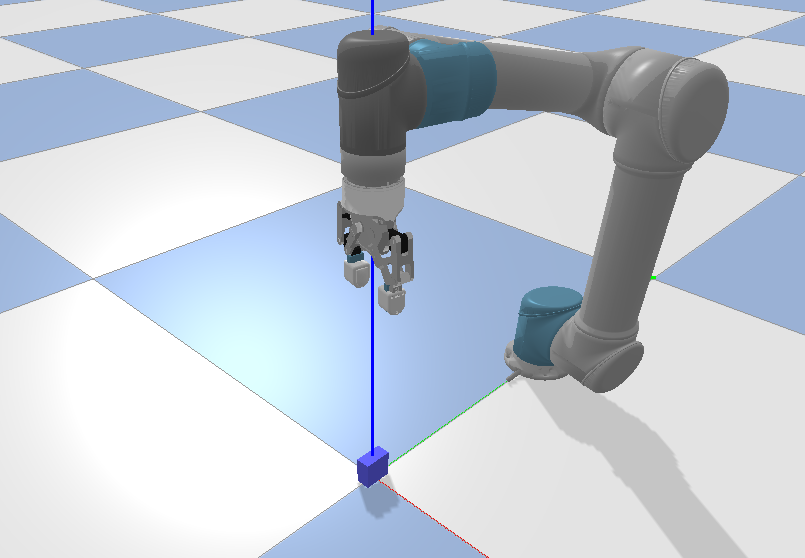
\includegraphics[width=0.47\textwidth]{docs/Project Report/Media/4_2_2_init_config.png}\label{fig:4.1a}}}%
    \qquad
    \subfloat[\centering Move end effector to specific pose (with vertical padding)]{{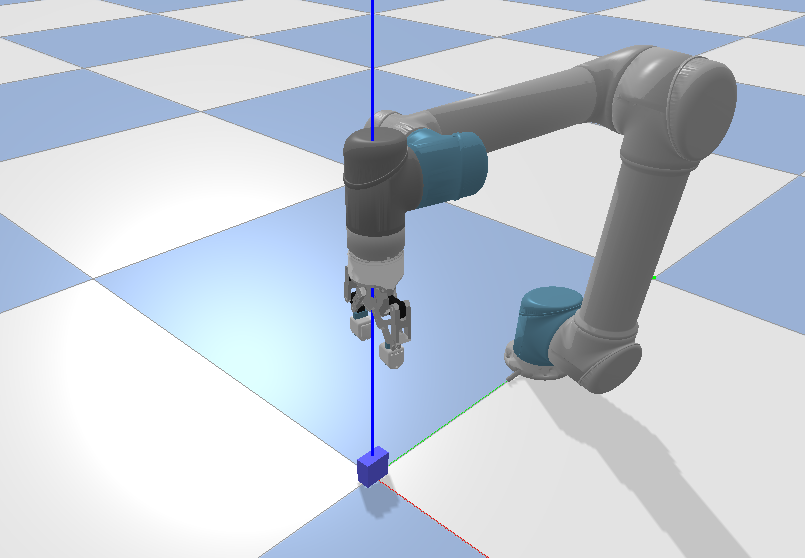
\includegraphics[width=0.47\textwidth]{docs/Project Report/Media/4_2_2_ee_pose_with_pad.png}\label{fig:4.1b}}}%
    \qquad
    \subfloat[\centering Remove vertical padding and close gripper]{{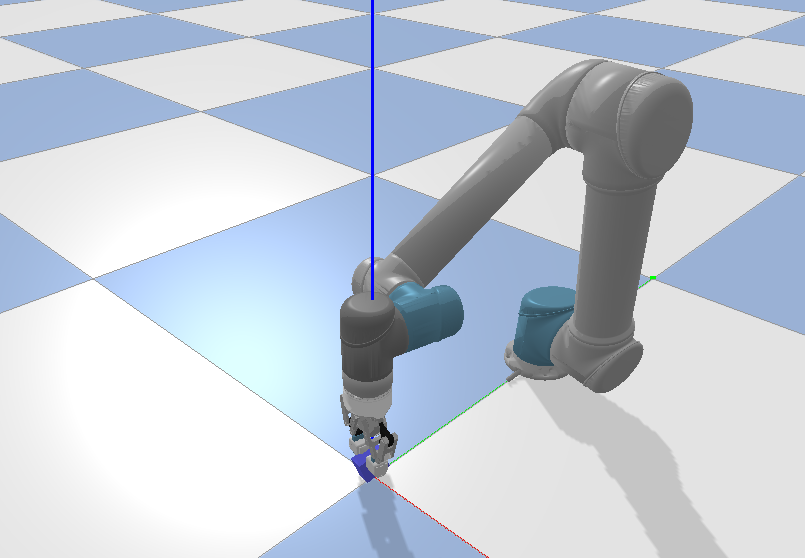
\includegraphics[width=0.47\textwidth]{docs/Project Report/Media/4_2_2_ee_pose_no_pad.png}\label{fig:4.1c}}}%
    \qquad
    \subfloat[\centering Lift object]{{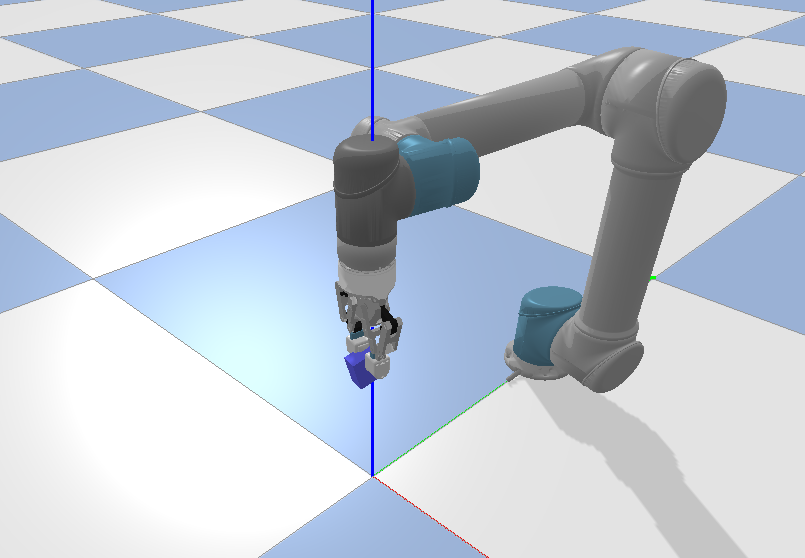
\includegraphics[width=0.47\textwidth]{docs/Project Report/Media/4_2_2_pick_obj.png}\label{fig:4.1d}}}%
    \caption{Tactile and visual data collection procedure on a single generated hand pose}%
    \label{fig:4.1}%
\end{figure}

Before lifting the object, the robot measures the number of contact points between the two fingers and the object to ensure the grasp is stable. We define a grasp to be stable if there are a non-zero number of contact points, in which the robot records depth and colour tactile information using the DIGIT \cite{Lambeta2020DIGIT} tactile sensors on each finger. We concatenate each pair of depth and colour tactile readings into a $(160\times240)$ grey-scale image and a $(160\times240\times3)$ RGB image respectively.\\

\newpage
Upon acquiring tactile readings, the robot executes a sanity check on the recorded tactile data from DIGIT cameras. The DIGIT cameras use a combination of depth sensing and colour imaging technologies to produce tactile readings. These cameras have a structured light system that projects a pattern of infrared light onto the object being touched. The camera then captures the reflected light and uses it to calculate the depth of the object at each pixel location. To produce colour tactile readings, the camera also includes a traditional RGB colour camera. This camera captures the colour information of the object at each pixel location. The depth and colour information is then combined to produce a textured 3D representation of the object's surface, which can be used to extract tactile features such as roughness, curvature, and shape. The following figure describes a set of depth-colour tactile readings collected from the DIGIT cameras via our simulation:
\begin{figure}[H]
    \centering
    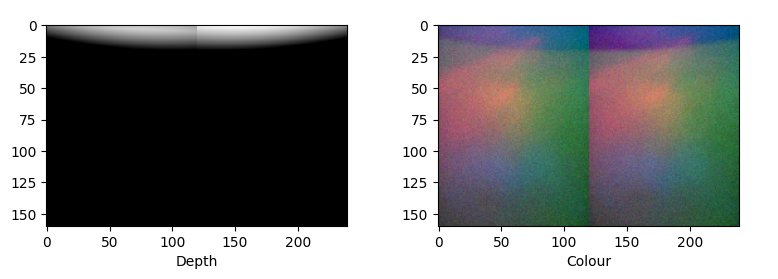
\includegraphics[width=0.8\textwidth]{docs/Project Report/Media/4_2_tactile_data_visualisation.png}
    \caption{Example depth and colour tactile readings collected from a DIGIT camera}
    \label{fig:4.2}
\end{figure}


After running the sanity check, we analyse the depth data exclusively, as the colour data is a mere RGB representation of the depth data, and thus does not require any additional scrutiny. This process involves assessing whether the average pixel value surpasses a predetermined threshold, thereby enabling the elimination of spurious signals (\hyperref[fig:4.3a]{Figure 4.3a}) and preserving the integrity of the precise depth data (\hyperref[fig:4.3b]{Figure 4.3b}). By implementing this approach, the quality of the data is significantly improved, thus ensuring the accurate lifting of the object.

\begin{figure}[H]%
    \centering
    \subfloat[\centering Invalid depth data]{{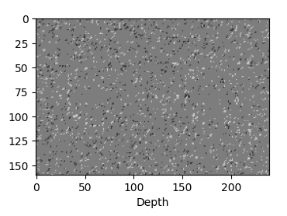
\includegraphics[width=0.45\textwidth]{docs/Project Report/Media/4_2_2_invalid_tactile_data.png}\label{fig:4.3a}}}%
    \qquad
    \subfloat[\centering Valid depth data]{{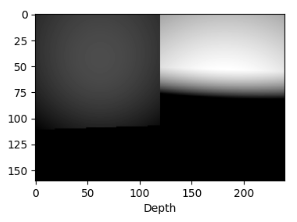
\includegraphics[width=0.45\textwidth]{docs/Project Report/Media/4_2_2_valid_tactile_data.png}\label{fig:4.3b}}}%
    \caption{Concatenated depth data for each finger}%
    \label{fig:4.3}%
\end{figure}

Once the robot verifies that the object is stably held (i.e. the tactile data is valid), it lifts the object vertically upwards by an offset of $p_z$ and holds the object for 750 steps (\hyperref[fig:4.1d]{Figure 4.1d}). Finally, the robot records a binary outcome of the grasp by determining if the change in the object's z-position $\Delta z$ is greater or equal to the vertical padding $p_z$:

\begin{equation}
    outcome=\begin{cases}1 & \Delta z\geq p_z \\ 0 & \Delta z<p_z\end{cases}
\end{equation}

After executing each random pose, we append the collected tactile data, end effector pose and grasp outcome to individual arrays. Once the required data for our $n$ random end effector poses has been collected, these arrays are saved to separate files which can be loaded for further analysis. Specifically, we create one .npy file each for the depth, colour, grasp outcomes, and random pose data.


\newpage
\section{Dataset Validation and Visualisation}\label{sec:4.3}
Before using the generated tactile and visual data for random hand configurations for analysis or modelling, it is important to validate and visualise it to ensure its quality and reliability. In this context, this article will explore the process of visualising and validating a dataset of tactile sensor readings and end-effector poses. We will discuss various techniques and tools that can be used to explore the data, identify patterns and anomalies, and ensure that it meets the requirements of the analysis or model being built. In this section, we explore our data to understand any underlying patterns or characteristics and prevent the generation of abnormal grasp data (as in \hyperref[fig:4.3]{Figure 4.3}).


\subsection{Visualising Tactile Data}\label{sec:4.3.1}
The tactile readings collected from our simulation are represented in the depth and colour images, as depicted in the figures below. These figures display the data for two grasp attempts - one successful (\hyperref[fig:4.4a]{Figure 4.4a}) and one unsuccessful (\hyperref[fig:4.4b]{Figure 4.4b}) - which were based on end effector poses randomly generated by the system. Furthermore, we present a 3D visualisation of the hand pose and the object, with the target object shown as a blue box and the gripper represented as a staple-like object consisting of two fingers.
\begin{figure}[H]%
    \centering
    \subfloat[\centering Successful grasp data]{{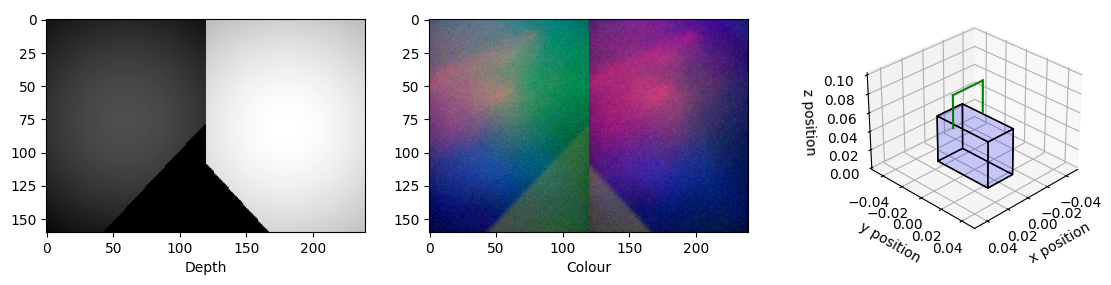
\includegraphics[width=\textwidth]{docs/Project Report/Media/4_3_successful_grasp_data.png}\label{fig:4.4a}}}%
    \qquad
    \subfloat[\centering Unsuccessful grasp data]{{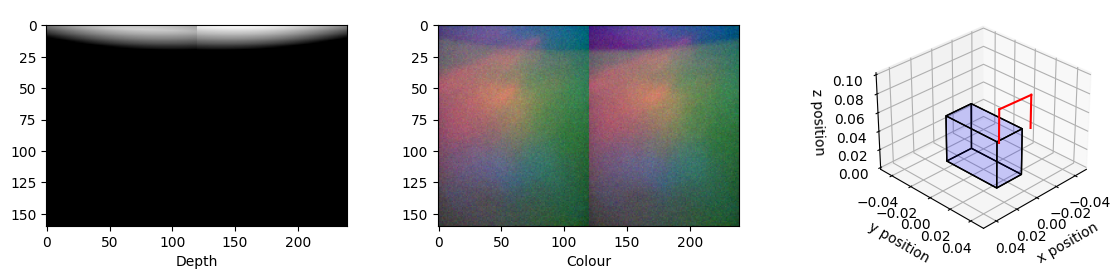
\includegraphics[width=\textwidth]{docs/Project Report/Media/4_3_unsuccessful_grasp_data.png}\label{fig:4.4b}}}%
    \caption{Left to right: Depth readings, Colour (RGB) readings, Skeleton 2-finger model to represent a hand pose}
    \label{fig:4.4}%
\end{figure}



\newpage
\subsection{Visualising Hand Poses}\label{sec:4.3.2}
We create a visualisation of each hand pose $X_n$ in a 3-dimensional space, using its Cartesian coordinates and the "pitch-roll-yaw" rotational matrix representation $R$ of its Euler angles ($\alpha,\beta,\gamma$) \cite{weisstein}:

\begin{equation}
    R=r_x\cdot(r_y\cdot r_z)
\end{equation}

\noindent where $r_x$, $r_y$ and $r_z$ are the rotational matrices about the $x$, $y$ and $z$-axis respectively:

\begin{figure}[H]
    \centering
    \begin{equation*}
        r_x = \begin{pmatrix}1&0&0 \\ 0&cos(\alpha)&sin(\alpha) \\ 0&-sin(\alpha)&cos(\alpha)\end{pmatrix}\;\;
        r_y = \begin{pmatrix}cos(\beta)&0&-sin(\beta) \\ 0&1&0 \\ sin(\beta)&0&cos(\beta)\end{pmatrix}\;\;
        r_z = \begin{pmatrix}cos(\gamma)&sin(\gamma)&0 \\ -sin(\gamma)&cos(\gamma)&0 \\ 0&0&1 \end{pmatrix}
    \end{equation*}
    \caption{Rotational matrices for each axis in the rotational matrix representation of Euler angles}
    \label{fig:4.5}
\end{figure}

\noindent Using this information, we annotate all randomly-generated hand poses from our dataset in 3 dimensions using \verb|matplotlib|. Each 6D hand pose is represented using a skeleton 2-finger model in a similar manner to \cite{Bekiroglu2012LearningTA}, where green and red poses denote successful and unsuccessful grasps respectively:
\begin{figure}[H]%
    \centering
    \subfloat[\centering Box without poses]{{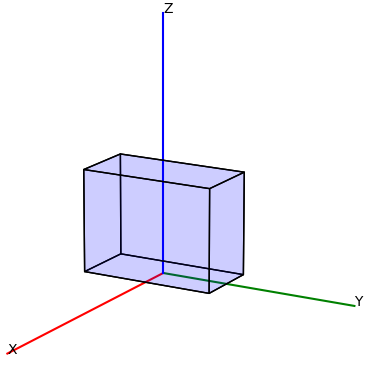
\includegraphics[width=0.29\textwidth]{docs/Project Report/Media/4_3_2_box_3d_plot.png} }}%
    \qquad
    \subfloat[\centering Orientation 1]{{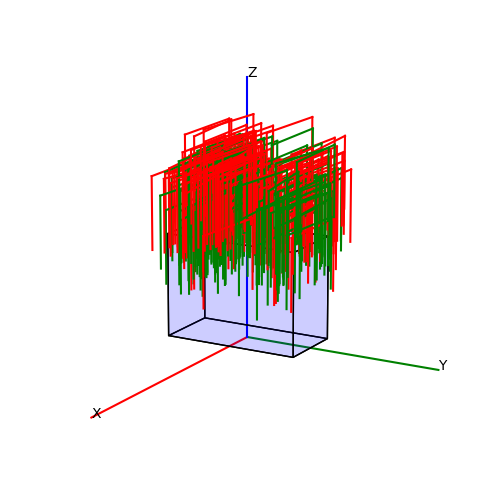
\includegraphics[width=0.29\textwidth]{docs/Project Report/Media/4_3_2_all_ee_pose_visualise.png} }}%
    \qquad
    \subfloat[\centering Orientation 2]{{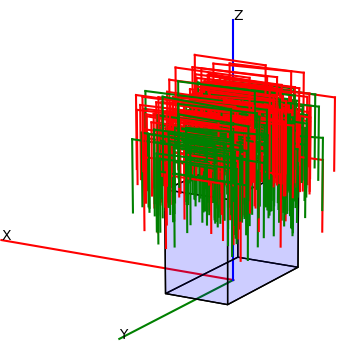
\includegraphics[width=0.29\textwidth]{docs/Project Report/Media/4_3_2_all_ee_pose_visualise2.png} }}%
    \caption{Visualisation of 200 random end effector poses}%
    \label{fig:4.6}%
\end{figure}


\newpage
\section{Feature Engineering \& Data Pre-processing}\label{sec:4.4}
We aim to assess the efficacy of utilising our multi-modal dataset for our grasping task by experimenting with various combinations of the tactile and visual (random end effector poses) data.


\subsection{Multi-modal Data Combinations}\label{sec:4.4.1}
Based on the tactile and visual data collected in section 4.2, we created different combinations of the dataset to determine the best representation for our analysis. The table below presents a summary of the various data combinations we tested and their corresponding creation methods.
\begin{table}[H]
    \centering
    \resizebox{\textwidth}{!}{%
        \begin{tabular}{ll p{10cm}}
            \toprule
            Data Combination & Dimensions & Creation \\
            \midrule
            Tactile only & $N\times160\times240\times4$ & Concatenating the depth ($N\times160\times240$) and colour ($N\times160\times240\times3$) data \\
            Visual only & $N\times6$ & Random 6D end effector poses \\
            Tactile + Visual & $N\times(160\times240\times4+6)$ & Concatenating the flattened tactile-only and visual-only datasets \\
            \bottomrule
        \end{tabular}
    }
    \caption{Dataset combinations}
    \label{tab:4.1}
\end{table}
The first dataset consists of tactile sensor readings collected from a robotic gripper during grasping tasks. The dataset has a shape of $N\times160\times240\times4$, with $N$ distinct concatenated colour and depth tactile sensory readings per finger collected from the simulation data collection pipeline (\ref{sec:4.2.2}). The following flowchart illustrates how the tactile dataset was created:
\begin{figure}[H]
    \centering
    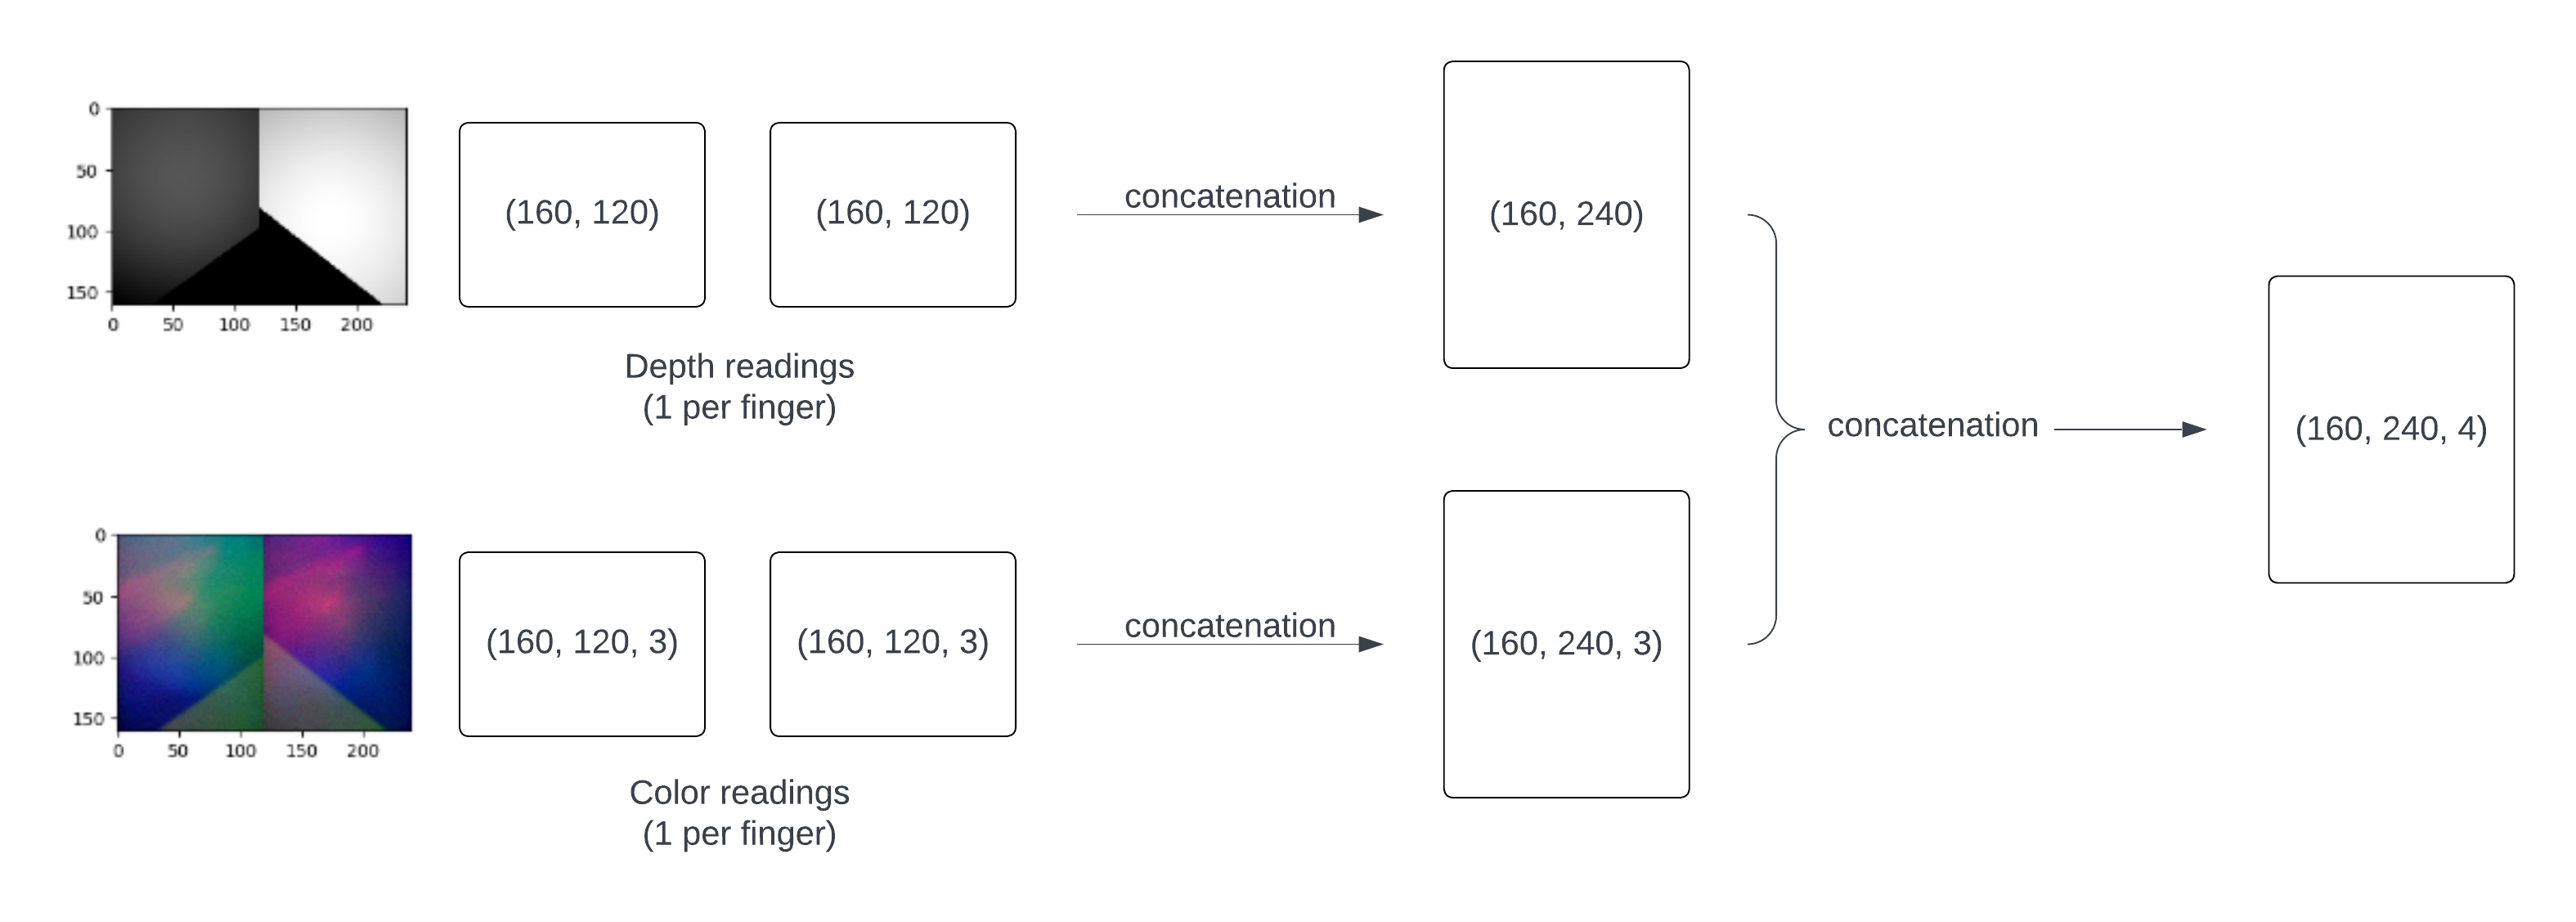
\includegraphics[width=\textwidth]{docs/Project Report/Media/4_4_1_tactile_dataset_creation.png}
    \caption{Creating the tactile dataset}
    \label{fig:4.7}
\end{figure}

The second dataset consists of end effector poses relative to the robot arm during grasping tasks. The dataset has a shape of $N\times6$, where $6$ represents the 6 degrees of freedom (DOF) of the simulation robot. We leave this dataset as it is.\\

The third dataset is a combination of tactile and visual data and consists of both tactile sensor readings and end effector poses collected during grasping tasks, concatenated together as NumPy arrays along the second dimension, creating a dataset of the shape $N\times(160\times240\times4+6)$.\\

Concatenation approaches involving the combination of sensory data for robotic grasping analysis have been explored in several related works. Calandra et al. (2018) \cite{Calandra_2018} used a combination of tactile and visual data to train a deep neural network for predicting grasp outcomes. The authors concatenated the tactile sensor readings and end effector poses into a single input vector for the neural network.


\subsection{Dimensionality Reduction}\label{sec:4.4.2}
In this project, we represent tactile sensory readings as images, specifically, grayscale for depth data and RGB for colour data. As the dimensionality of this data has a significant impact on computational costs, we have employed dimensionality reduction techniques to alleviate this issue, including principal component analysis (PCA) and convolutional neural networks (CNN) for feature extraction.


\subsubsection{Principal Component Analysis (PCA)}\label{sec:4.4.2.1}
PCA is a widely used linear technique that projects the high-dimensional input data onto a lower-dimensional space, capturing the maximum amount of variance in the data with fewer dimensions. By reducing the dimensionality of the data, PCA can facilitate more efficient computation and enable the extraction of meaningful patterns and features from the data.\\

PCA is particularly useful for concatenated tactile and visual data, as it can extract relevant features from both modalities and combine them to form a lower-dimensional representation of the data. For example, PCA can be used to extract principal components that represent the most significant tactile and visual features, which can then be combined to form a lower-dimensional representation of the data. The resulting representation can be used as input to machine learning algorithms for classification or regression tasks.\\

It is worth noting that the effectiveness of PCA for dimensionality reduction depends on several factors, such as the number of input dimensions, the amount of variance in the data, and the distribution of the data. Additionally, the choice of the number of principal components to retain can also impact the performance of the method. Hence, a careful evaluation of the effectiveness of PCA for the given task is necessary, including the selection of an appropriate number of principal components to retain, and any trade-offs between computation time and performance.


\subsubsection{Convolution Neural Network (CNN) Feature Extraction}\label{sec:4.4.2.2}
In the context of multi-modal sensor data, feature extraction using convolutional neural networks (CNNs) has gained popularity due to their ability to capture spatial and temporal patterns in the data. The CNN architecture, as described with interleaved convolution and pooling layers, is well-suited for detecting local features in the input data. The convolution layers extract low-level features, such as edges or textures, while the pooling layers help reduce the dimensionality of the feature maps and provide translational invariance to the learned features. The combination of these layers can create a hierarchy of feature representations, with higher-level features capturing more complex and abstract patterns in the data.

\begin{figure}[H]
    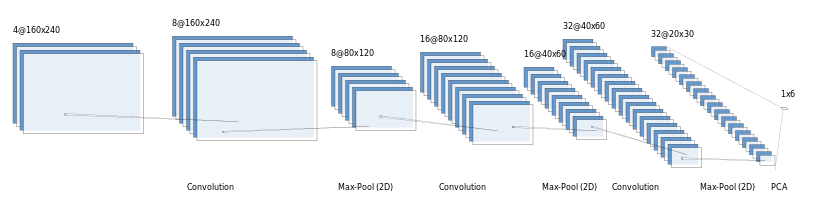
\includegraphics[scale=0.7]{docs/Project Report/Media/4_4_2_nn.png}
    \caption{Architecture for feature extraction CNN}
    \label{fig:4.8}
\end{figure}

\hyperref[fig:4.8]{Figure 4.8} visualises the specific CNN architecture used in the baseline, consisting of three convolutional layers interleaved with MaxPool2D layers with a 2 × 2 kernel, which is effective in capturing features from concatenated tactile and visual sensory data. 


\subsection{Data Pre-processing}\label{sec:4.4.3}
Normalisation of data prior to model training is a well-established practice in machine learning, known to improve the accuracy and efficiency of the learning process. In the context of tactile sensor readings and end effector poses, normalisation is particularly relevant due to the large differences in the scale of the data. For instance, RGB pixel values for the colour dataset vary between 0 to 255, while Euler angles in the hand pose dataset vary between $-\pi$ and $\pi$.\\

Failure to normalise the data can result in numerical instability, as differences in scale can cause the weights of the model to become disproportionately small or large, thereby hampering effective learning. Moreover, normalisation can improve model generalisation by reducing the impact of outliers and mitigating the effects of varying ranges of feature values in the data. Finally, normalisation facilitates comparison of the relative importance of different features, thereby enabling the identification of the most significant ones and elimination of redundant or less important ones.


\section{Model Training}\label{sec:4.5}
To train the binary logistic regression classifier on the tactile sensory data and end effector poses, an 80-20 split was used with the \verb|train_test_split()| function provided by the \verb|sklearn| library. The training set consisted of 80\% of the data, while the remaining 20\% was utilised for validation. The model was trained using the \verb|sklearn| logistic regression implementation, which provided flexibility in setting the hyper-parameters such as the solver type and regularisation method. However, regularisation was not applied in this training process considering the high dimensionality of the dataset.\\

After preparing the datasets, the logistic regression (logit) classifier was trained using the three dataset combinations that were previously discussed in \hyperref[sec:4.4.1]{Section 4.4.1}. To further explore the dataset characteristics, a combination of dimensionality reduction techniques was applied to these datasets, as discussed in \hyperref[sec:4.4.2]{Section 4.4.2}. Specifically, the techniques used were ConvNet only and ConvNet with PCA (top $k$ principal components). The logit model was then trained on these variations of the datasets with the aim of selecting the model and dataset combination that achieves the best accuracy. This approach allowed us to thoroughly explore the impact of different dataset combinations and dimensionality reduction techniques on the performance of the logit classifier.


\subsection{Summary of training results}\label{sec:4.5.1}
\label{sec:4.5.1}
\begin{table}[H]
    \centering
    \small
    \begin{tabular}{lccccc}
        \toprule
        & \multicolumn{3}{c}{Dataset} & \multicolumn{2}{c}{Property of sample} \\
        \cmidrule{2-4}\cmidrule{5-6}
        Pre-processing & Visual only & Tactile only & Both & Shape & Dimensionality \\
        \midrule
        Raw & 70.83\% & 83.33\% & 83.33\% & 160x240x4 & 153600 \\
        CNN & -- & 83.33\% & 87.50\% & 64x10x15  & 9600 \\
        CNN + PCA ($k=5$) & -- & 77.08\% & 77.08\% & 5 & 5\\
        \bottomrule
    \end{tabular}
    \caption{Accuracy of LR model on dataset variations}
    \label{tbl:4.2}
\end{table}
As previously discussed, the logistic regression model was trained on three different dataset segmentations and three pre-processing methods were applied. The results, as presented in \hyperref[tbl:4.2]{Table 4.2}, indicate that although utilising ConvNets and/or PCA techniques did not have a significant impact on the accuracy of the logit model, it is noteworthy that the dimensionality of the datasets was significantly reduced by more than 90\% when dimensionality-reducing techniques were used.


\subsection{Trade-off between accuracy and dimensionality}\label{sec:4.5.2}
Compared to traditional techniques like PCA, CNNs can learn complex, non-linear relationships between the tactile and visual features and the grasp outcome. This is particularly useful when dealing with high-dimensional data, where PCA may not capture the underlying patterns in the data. Moreover, the ability of CNNs to learn hierarchical feature representations can make them more interpretable, as each layer captures increasingly complex and abstract features, leading to a better understanding of the underlying mechanisms of the problem.


\section{Conclusion}\label{sec:4.6}
Based on the results presented in \hyperref[tbl:4.2]{Table 4.2}, we have determined that using both tactile and visual data together produces the highest accuracy for our LR models. While raw data performed better than other pre-processing techniques, we recognise that the dimensionality of the data must also be considered. Therefore, we have found that extracting features from our dataset using a ConvNet and selecting only the top $k=5$ components provides comparable accuracy with significantly lower dimensionality.



%----------------------------------------------------------------------------------
% Section 5: Proposed Approach
%----------------------------------------------------------------------------------
\chapter{Multilayer Perceptron for Grasp Stability Prediction}\label{chap:5}
Achieving successful grasping of objects in a robotic environment is challenging due to the high-dimensional, noisy, and uncertain nature of the task, which requires accurate perception, planning, and control. To address this issue, we propose a multilayer perceptron (MLP) neural network that predicts the grasp stability label of an end effector pose. MLPs are feed-forward neural networks consisting of at least three fully-connected layers of perceptrons, including an input layer for receiving input data, an output layer for producing a prediction, and at least one hidden layer that enables the MLP to learn complex representations of the data. Our proposed approach is specifically designed to identify grasp configurations that yield high stability and success rates for specific objects, a critical task in robotic grasping.\\

MLPs are well-suited to learn non-linear relationships between input and output data, making them suitable for identifying patterned configurations from complex datasets and generalising simple grasping strategies for different object types. For example, grasping an object around its centre of gravity can minimise rotational forces that could cause it to tilt and increase the likelihood of a successful grasp. In this context, our MLP-based approach extracts important features from tactile and visual data using an identical Convolutional Neural Network architecture, from which we select the top five principal components to represent the extracted features.\\

To evaluate the performance of our model, we conducted several experiments on different primitive object types, including rectangular boxes, cylinders, and bottle-shaped objects (which are more rigid than typical cylinders), to assess the robustness of the model towards various objects. Additionally, we tested whether the model is able to generalise simple grasping strategies per object type. We compared the performance of our model with state-of-the-art methods for predicting grasp stability, including baseline methods on hand-engineered features and other neural network-based models \cite{mahler2017dexnet, 7487517}.\\

In the following sections, we provide a detailed description of our approach, experimental setup, and results, and discuss the implications of our work in the field of robotic grasping.


\section{Related Work}\label{sec:5.1}
There have been several academic studies addressing the problem of grasp stability classification using neural networks. In this section, we will briefly review some of these works. Kumra and Kana (2017) \cite{8202237} presented a novel approach to grasp detection that predicts an optimal grasping pose using RGB images of a scene. Their method considers the robotic grasp detection problem as finding a successful grasp configuration for a given object image. To address this, they proposed a single-step prediction technique, which is faster and less computationally expensive compared to previous methods that rely on running a simple classifier multiple times on small image patches.
\begin{figure}[H]
    \centering
    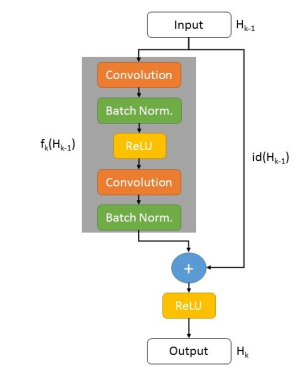
\includegraphics[width=0.4\textwidth]{docs/Project Report/Media/5_1_kumra_kana_2017_residual_block.png}
    \caption{Kumra and Kanan \cite{8202237}: Robotic Grasp Detection using Deep Convolutional Neural Networks: Example of a residual block in ResNet}
    \label{fig:5.1}
\end{figure}
To solve the grasp detection problem, the authors used ResNet-50, a 50-layer deep residual model (see \ref{fig:5.1}) that incorporates residual layers to reformulate the mapping function between layers and overcome the challenge of learning an identity mapping. The authors introduced two different architectures for robotic grasp prediction: a uni-modal grasp predictor that uses only single-modality information such as RGB, and a multi-modal grasp predictor that uses multi-modal information such as RGB and depth.\\


Mahler et al. \cite{mahler2017dexnet} have proposed a method for evaluating grasp quality using a CNN trained on RGB-D images and force measurements. RGB-D refers to a type of sensor that captures both colour (RGB) and depth (D) information about a scene. RGB-D sensors typically consist of a regular colour camera to capture RGB images and an additional depth sensor, such as a time-of-flight or structured light sensor, which provides a depth image. The combination of RGB and depth information can be particularly useful for robotics applications, as it allows the robot to perceive and reason about the 3D structure of the environment, and to distinguish between objects that are close together but at different depths.\\

In this paper, the authors propose a method for evaluating grasp quality using a CNN trained on RGB-D images and force/torque measurements. The network takes as input an RGB-D image of the scene, along with the 6-dimensional force/torque measurements recorded during a grasp attempt. It then predicts a scalar value for each grasp, indicating its expected success rate. The CNN was trained on a dataset of over 10000 grasps on a variety of objects. However, a limitation of this approach is that it requires accurate force sensing during the grasp attempt, which may not be always feasible in practice. Additionally, the scalar success rate predicted by the network may not be as interpretable as other grasp stability metrics, such as the wrench space analysis or the friction cone model. Nonetheless, this paper represents an important step towards using neural networks to evaluate grasp quality in robotics applications.


\newpage
\section{Methodology}\label{sec:5.2}
In this section, we describe the methodology used to train and evaluate our proposed approach for predicting grasp stability using a multilayer perceptron (MLP) neural network. We begin by presenting the dataset we used, which consists of tactile and visual data collected from a variety of objects, along with ground-truth labels indicating whether each grasp was successful or not. We then describe the architecture of our MLP model, including the number and size of the layers, the activation functions used, and any regularisation techniques employed. Next, we explain the training procedure used to optimise the model's weights, including the optimisation algorithm used, the learning rate schedule, the batch size, and the number of epochs. We then describe the evaluation metrics used to assess the performance of our model, along with the baseline methods against which we compared it. Finally, we present the results of our experiments and discuss their implications for the field of robotic grasping.


\subsection{Dataset Collection}\label{sec:5.2.1}
Utilising our Pybullet data collection pipeline from \hyperref[sec:4.2.2]{Section 4.2.2}, we collect multi-modal data for every object variation. Then, for each variation, we manually select $i=4$ seed poses and record the data of 20 successful and 20 unsuccessful grasps with Gaussian noise applied to the seed pose. This creates a dataset of 9x160=1440 grasps in total (720 stable and 720 unstable grasps) consisting of tactile sensor readings and hand poses.


\subsection{Primitive Objects and Variations}\label{sec:5.2.2}
To enhance the robustness of our model, we have trained it on three primitive object categories that collectively represent a sizeable proportion of daily-life objects: rectangular boxes, cylinders and bottles. For each object category, we generate three instances with slightly different dimensions. The 3D meshes of these object variations and their dimensions are listed in \hyperref[tbl:5.1]{Table 5.1}.

\begin{table}[H]
    \centering
    \resizebox{\textwidth}{!}{%
        \begin{tabular}{lccccccccc}
            \toprule
            & 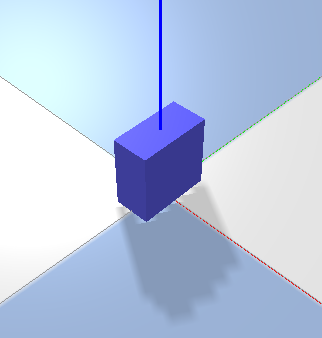
\includegraphics[width=0.1\textwidth]{docs/Project Report/Media/block1.png} & 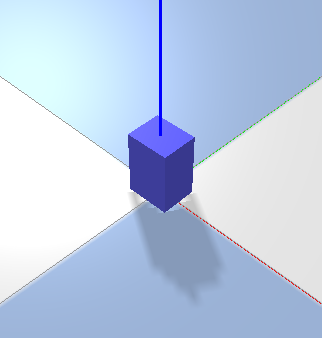
\includegraphics[width=0.1\textwidth]{docs/Project Report/Media/block2.png} & 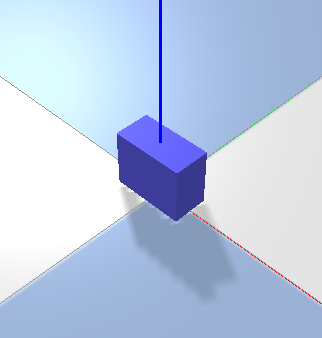
\includegraphics[width=0.1\textwidth]{docs/Project Report/Media/block3.png} &
            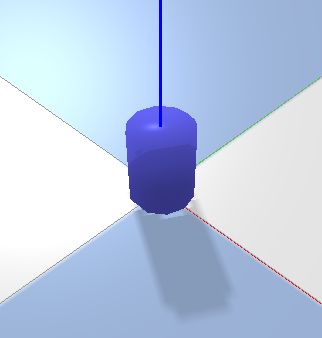
\includegraphics[width=0.1\textwidth]{docs/Project Report/Media/cylinder1.png} & 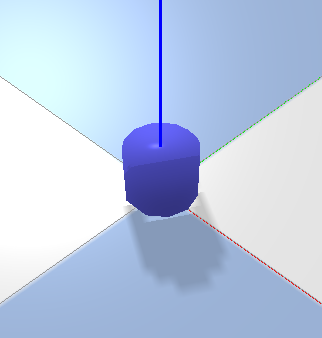
\includegraphics[width=0.1\textwidth]{docs/Project Report/Media/cylinder2.png} & 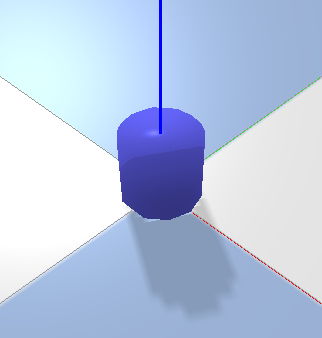
\includegraphics[width=0.1\textwidth]{docs/Project Report/Media/cylinder3.png} & 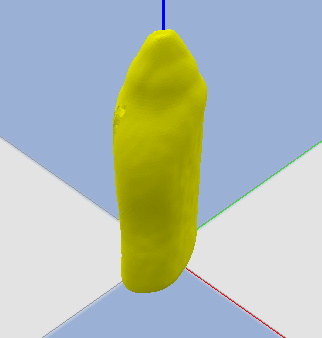
\includegraphics[width=0.1\textwidth]{docs/Project Report/Media/mustard_bottle1.png} & 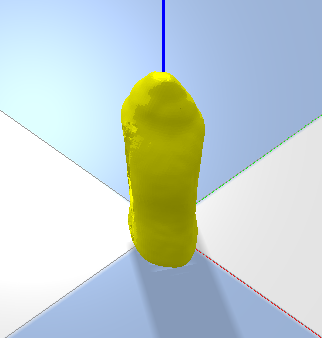
\includegraphics[width=0.1\textwidth]{docs/Project Report/Media/mustard_bottle2.png} &  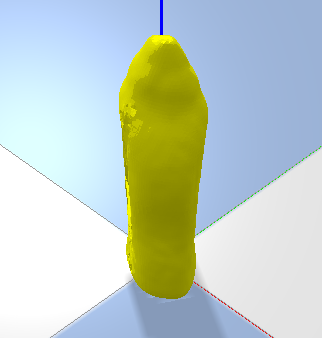
\includegraphics[width=0.1\textwidth]{docs/Project Report/Media/mustard_bottle3.png} \\
            & Box 1 & Box 2 & Box 3 & Cylinder 1 & Cylinder 2 & Cylinder 3 & Bottle 1 & Bottle 2 & Bottle 3 \\
            \midrule
            Depth  & 0.025 & 0.03  & 0.05  & 0.04 & 0.045  & 0.05  & 0.06 & 0.04 & 0.04 \\
            Width  & 0.05  & 0.025 & 0.025 & 0.04 & 0.045  & 0.05  & 0.04 & 0.06 & 0.06 \\
            Height & 0.05  & 0.045 & 0.04  & 0.05 & 0.035  & 0.045 & 0.04 & 0.06 & 0.04 \\
            Radius & --    & --    & --    & 0.02 & 0.0225 & 0.025 & --   & --   & --   \\
            \bottomrule
        \end{tabular}
    }
    \caption{3D meshes of all experimental object variations}
    \label{tbl:5.1}
\end{table}


\subsection{Introducing Geometric Features of Objects}\label{sec:5.2.3}
In this section, in addition to the end effector poses in our visual dataset, we investigate the possible impact and improvement of introducing geometric features of objects on our MLP model. Each primitive object category in our dataset possesses unique characteristics. For instance, the curvature of an object's surface can differentiate cylinders and bottles from boxes with ease. As objects within a primitive class often share similar geometric features (such as the curvature of cylinders), our model could potentially generalise successful and unsuccessful grasp poses within each object category by establishing a connection between those poses and the object's properties.\\

To this end, we extracted and analysed several geometric features of each of the 9 object variations in order to determine which of them can effectively differentiate between the object categories. We conclude that principal curvatures best represent the geometric features of said objects.


\subsubsection{Principal Curvature}\label{sec:5.2.3.1}
The principal curvatures of an object mesh are pair of maximum and minimum values of curvatures at each vertex of the mesh, expressed by the eigenvalues of the shape operator at that vertex \cite{enwiki:1141654906}. We investigate whether the top $k$ principal curvatures are able to categorize the object variations correctly.

\begin{figure}[H]
    \centering
    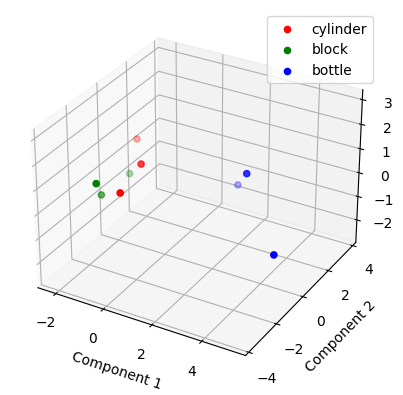
\includegraphics[width=0.4\textwidth]{docs/Project Report/Media/5_2_3_principal_curvature_3d.png}
    \caption{Clustering using PCA-extracted components based on principal curvatures of objects}
    \label{fig:5.2}
\end{figure}

\hyperref[fig:5.2]{Figure 5.2} visualises the top $k=2$ and $k=3$ principal curvatures for all the object variations in our dataset. We found that the principal curvatures were able to:
\begin{enumerate}[\itemsep=0em]
    \item capture a high amount of variance of the curvatures for all objects
    \item successfully cluster the object variations for each category
\end{enumerate}


\subsubsection{Other Features}\label{sec:5.2.3.2}
In addition to principal curvatures, we attempted to extract convexity and fundamental dimensions of objects, aimed at capturing their size and shape characteristics. Despite the analytical efforts, the results obtained from these features were not deemed promising and therefore were not incorporated into the model. Consequently, it can be inferred that the principal curvatures hold significant potential as a valid representation of geometric features for the object dataset under consideration.


\subsection{Dataset Pre-processing}\label{sec:5.2.4}
Based on the analysis results of our baseline approach in \hyperref[sec:4.7]{Section 4.7}, we concluded that under limited dimensionality circumstances, the Logistic Regression model fits the dataset with the highest accuracy using a convolutional neural network as a dimensionality reduction technique. Therefore, before training our MLP, we extract important features from our dataset using the same CNN architecture as \ref{sec:4.4.2.2}. This results in a condensed dataset of shape $N\times512$ with $N$ examples. To improve the convergence speed and performance for training our MLP model, we normalise the tactile and visual datasets with zero mean and unit variance. This also prevents the initialisation of large weights during back-propagation.


\subsection{MLP Overview and Architecture}\label{sec:5.2.5}
We define our MLP model in PyTorch and tailor it to predict grasp stability labels given a varying dataset size (depending on the dataset combination we use). This is achieved by dynamically declaring the input size of the network through its \verb|input_size| parameter, allowing it to accommodate different dataset combinations for training. The MLP architecture consists of three fully connected layers, including two hidden layers with ReLU activation functions, and an output layer without an activation function.
\vspace{-0.2cm}
\begin{figure}[H]
    \centering
    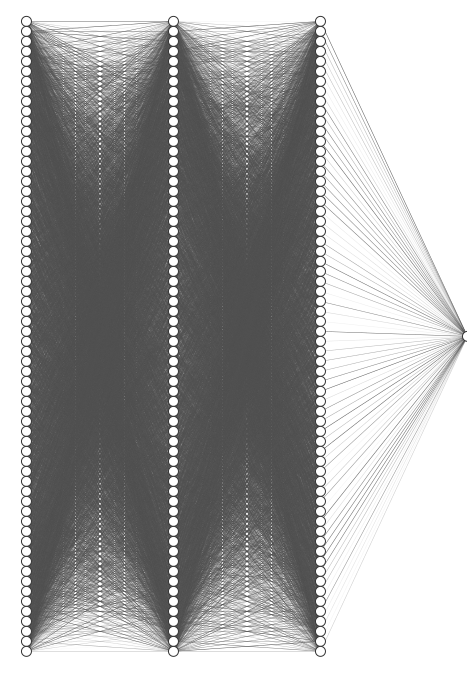
\includegraphics[width=0.25\textwidth]{docs/Project Report/Media/5_2_5_mlp_architecture.png}
    \caption{3-Layer MLP architecture. The input size of the model is flexible depending on the dimensions of the input dataset (the input size in the figure is 64 neurons for simplicity). The remaining layers consist of 64 neurons. The MLP outputs a binary label in the output layer, corresponding to the grasp stability prediction.}
    \label{fig:5.3}
\end{figure}


\section{Experiments on Impacts of Various Features}\label{sec:5.3}
In this section, we present the results of some additional experiments that evaluate the robustness of the MLP model to primitive object classes and the influence of sample size on the model's performance.


\subsection{Robustness of MLP Model to Primitive Object Classes}\label{sec:5.3.1}
To test the robustness of the MLP model to each primitive object class (rectangular box, cylinder, bottle), we trained the MLP model on two of its object variations and tested it on the remaining variation. The results are shown in the following table:
\begin{table}[H]
    \centering
    \small
    \begin{tabular}{llcc}
        \toprule
        Training Objects & Testing Object & Accuracy Mean (\%) & Accuracy Std. (\%) \\
        \midrule
        Box 1, Box 2 & Box 3 & 51.70 & 1.08 \\
        Box1, Box 3 & Box 2 & 67.80 & 2.65 \\
        Box2, Box 3 & Box 1 & 56.22 & 2.20 \\
        Bottle 1, Bottle 2 & Bottle 3 & 53.96 & 1.15 \\
        Bottle 1, Bottle 3 & Bottle 2 & 56.98 & 0.64 \\
        Bottle 2, Bottle 3 & Bottle 1 & 50.31 & 0.60 \\
        Cylinder 1, Cylinder 2 & Cylinder 3 & 53.46 & 1.05 \\
        Cylinder 1, Cylinder 3 & Cylinder 2 & 57.74 & 2.04\\
        Cylinder 2, Cylinder 3 & Cylinder 1 & 59.00 & 1.50 \\
        \bottomrule
    \end{tabular}
    \caption{Mean and standard deviation of MLP accuracy (\%) by object class across 5 trials}
    \label{tab:5.2}
\end{table}
As evident from our analysis, the MLP model's precision experienced a considerable decrement in performance when compared to its training on all object variations. This observed incongruity in model output can be ascribed to the deficiency of geometric features in distinguishing between different object variations belonging to the same object class. That is, the principal curvatures prove inadequate in encapsulating intra-class object variability, but rather effectively represent the variation exhibited between different object classes. This outcome is not unexpected, as our MLP is primed to forecast grasp stability labels for all primitive object types.


\subsection{Influence of Sample Size of Randomly-Shuffled Dataset on Model Performance}\label{sec:5.3.2}
This experiment aims to investigate the effect of sample size on the accuracy of our MLP model. Specifically, this approach aims to achieve a balance between the size of the training dataset, which is randomly shuffled without duplication prior to model training, and the desired accuracy of the model to mitigate the occurrence of overfitting or underfitting. The investigation of the impact of sample size on the accuracy of the MLP models may also yield valuable insights into the generalisability and robustness of the model.\\

In general, as the size of the training data set increases, the performance of the MLP model improves due to its ability to learn more complex patterns in the data. However, adding more data may also increase the computational cost of training the model, and there may be a point of diminishing returns where adding more data does not lead to a significant improvement in accuracy. Moreover, if the size of the dataset is too small, the MLP model may suffer from overfitting, which occurs when the model learns to fit the training data too closely and is unable to generalise well to new data.
\begin{figure}[H]
    \centering 
    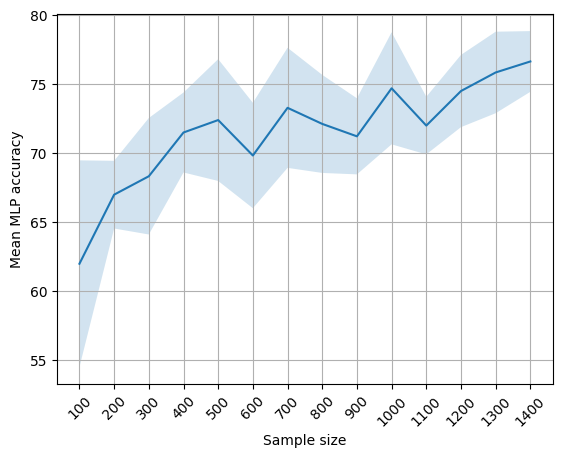
\includegraphics[width=0.6\textwidth]{docs/Project Report/Media/5_3_2_exp2_plot.png}
    \caption{Impact of the sample size of the randomised dataset on MLP accuracy}
    \label{fig:5.4}
\end{figure}
As depicted in \hyperref[fig:5.4]{Figure 5.4}, the accuracy of the MLP models increases with an increase in the sample size of the randomised dataset, which aligns with theoretical expectations.


\section{Training and Evaluation of Initial Results}\label{sec:5.4}
In this section, we explore the effectiveness of our Multi-Layer Perceptron (MLP) model in predicting grasp stability labels. Three distinct training methods were implemented and evaluated using the same dataset discussed in \hyperref[sec:5.2.2]{Section 5.2.2}.\\

The first method trained the MLP model on the aforementioned dataset to establish a baseline for its predictive performance. Subsequently, in the second method, the MLP model was trained on the same dataset concatenated with object features for each of the 9 object variations. This was done to investigate the impact of object features on the model's predictive performance. Finally, the third method involved applying Principal Component Analysis (PCA) to the dataset and re-training the MLP model with an input size of 5 principal components. This approach aimed to explore the effectiveness of dimensionality reduction in enhancing the model's accuracy.\\

Our dataset from \hyperref[sec:5.2.4]{Section 5.2.4} was split into training and validation sets with an 80:20 ratio using the \verb|train_test_split()| function. The MLP model was trained using the Binary Cross-Entropy (BCE) logit loss function, which is commonly employed in binary classification tasks, and the Adam optimiser, a popular optimisation algorithm for training neural networks, with a learning rate of 0.001. The BCE logit loss function measures the difference between the predicted output of the model and the true label, penalising the model more for predicting the wrong label with high confidence. On the other hand, the Adam optimiser combines the benefits of two other optimisation methods: AdaGrad and RMSProp.\\

The validation set was used to evaluate the performance of the trained MLP model on unseen data. The results of the study are indicative of the effectiveness of the proposed training method in predicting grasp stability labels. The model's generalisation ability was assessed by validating it on unseen data, ensuring that it did not over-fit the training data.


\subsection{Evaluation of Results}\label{sec:5.4.1}
Our model is primarily trained on the dataset consisting all data sources, that is, tactile and visual (end effector poses and geometric data). For comparison of its effectiveness, we also train it on other variations of the datasets. The results are as follows:
\begin{table}[H]
    \centering
    \small
    \begin{tabularx}{\textwidth}{c *6{>{\Centering}X}}
        \toprule
        & \multicolumn{5}{c}{Models} \\
        \cmidrule{2-6}
        & Tactile only & Visual only (without geometric) & Visual only (with geometric) & Both (tactile, visual) & Full (tactile, visual, geometric) \\
        \midrule
        Trial 1 & 72.57 & 63.54 & 61.46 & 74.74 & 75.69 \\
        Trial 2 & 68.75 & 59.03 & 62.85 & 70.57 & 74.65 \\
        Trial 3 & 69.10 & 66.32 & 62.85 & 75.08 & 75.35 \\
        Trial 4 & 70.49 & 56.94 & 62.85 & 76.12 & 70.14 \\
        Trial 5 & 72.92 & 56.60 & 60.42 & 74.74 & 78.12 \\
        \midrule
        Mean    & 70.77 & 60.49 & 62.09 & 74.25 & 74.79 \\
        Std.    & 1.72  & 3.83  & 0.99  & 1.91  & 2.60  \\
        \bottomrule
    \end{tabularx}
    \caption{Mean and standard deviations (std) of accuracies (\%) of various MLP models}
    \label{tbl:5.3}
\end{table}
The results indicated that adding object features to the dataset marginally improved the MLP model's predictive accuracy. Based on these results, we attempt to apply PCA to the complete dataset and reduce the input size to 5 principal components. \hyperref[fig:5.4]{Figure 5.4} shows the accuracies of our MLP model on varying numbers of principal components $k$ from applying PCA across 5 separate trials:
\begin{figure}[H]
    \centering
    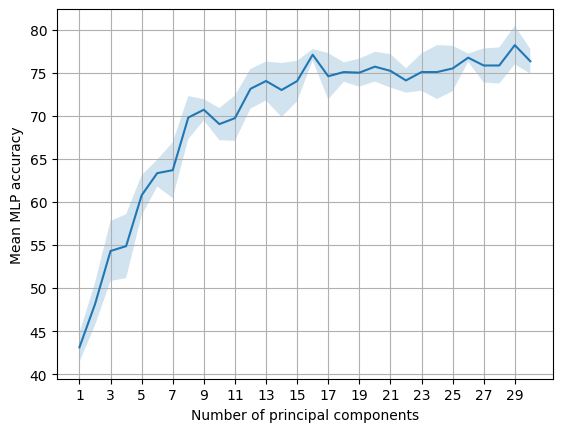
\includegraphics[scale=0.55]{docs/Project Report/Media/5_4_1_mlp_pca_accuracy_analysis.png}
    \caption{Investigating the impact of number of principal components $k$ on the mean MLP validation accuracy across 5 trials}
    \label{fig:5.5}
\end{figure}
This experimentation concludes that $k=21$ principal components results in the attainment of the most elevated mean validation accuracy (76.46\% on average, over five trials) utilising our MLP model. This selection represents a judicious choice, as it reduces the dimensionality of our dataset from (1440, 512) to (1440, 21), while concurrently preserving and even enhancing the general level of accuracy. As a reference point, we include in the following table a summary of the outcomes of several exemplary studies in the realm of grasp stability prediction, for the purpose of benchmarking our model's performance.

\begin{table}[H]
    \centering
    \small
    \renewcommand{\arraystretch}{1.5}
    \begin{tabular}{p{0.325\textwidth} p{0.175\textwidth} p{0.1\textwidth} p{0.15\textwidth} p{0.1\textwidth}}
        \toprule
        Paper & Type of Data & Dataset Size & Approach & Accuracy \\
        \midrule
        Learning to Predict Grasp Stability using Tactile and Proprioceptive Data, Zhang et al. (2020) & Tactile, proprioceptive & 1100 & Multi-modal deep neural network & 91.7\% \\
        Combining 3D Shape and Spatial-Temporal Features for Robust Grasp Stability Prediction, Jang et al. (2020) & Tactile (depth), force/torque & 7500 & Convolutional LSTM neural network & 87.5\% \\
        Object-Level Grasp Stability Prediction using Multimodal Deep Learning, Cao et al. (2019) & Tactile (depth), force/torque & 4500 & Multi-modal deep neural network & 87.3\% \\
        Grasp Stability Prediction using Multi-Modal Sensor Data and Graph Convolutional Networks, Veiga et al. (2020) & Tactile (depth), force/torque & 1500 & Graph convolutional network & 86.5\% \\
        A Comparative Study of Grasp Stability Prediction using RGB-D and Tactile Data, Li et al. (2021) & Tactile & 2500 & Multi-modal deep neural network & 88.2\% \\
        Data-Driven Grasp Stability Prediction with Probabilistic Contact Analysis, Wang et al. (2021) & Force/torque, object geometry & 10000 & Probablistic contact model with deep neural network & 82.6\% \\
        Predicting Grasp Stability using Multi-Modal Sensing and Deep Learning, Ren et al. (2020) & Tactile, force/torque & 3000 & Multi-modal deep neural network & 84.1\% \\
        Grasp Stability Prediction using Force and Tactile Sensors with Convolutional Neural Networks, Morales et al. (2018) & Tactile, force/torque & 2000 & CNN & 80.5\% \\
        Grasp Stability Prediction using Object Geometry and Force-Torque Sensing, Marin et al. (2021) & Force/torque, object geometry & 12000 & SVM & 76.7\% \\
        Grasp Stability Prediction using Vision-based Features and Gaussian Processes, Tang et al. (2018) & Tactile (depth), object geometry & 1500 & Gaussian processes & 77.1\% \\
        \bottomrule
    \end{tabular}
    \caption{Comparison of performance of various academic works on grasp stability prediction}
    \label{tbl:5.4}
\end{table}


\subsection{Limitations}\label{sec:5.4.2}
This study was subject to a limitation that warrants acknowledgement, specifically, the relatively modest sample size of the dataset we collected. This shortcoming may have exerted an impact on the accuracy of our findings. The source of this limitation is primarily attributed to the data collection pipeline in Pybullet, which demands a substantial amount of time to gather adequate data for the purpose of training. This arises from our approach of generating random hand configurations for grasping, and imposing constraints on the collection process to yield a balanced dataset (namely, an equal number of successful and unsuccessful grasps).

\section{Conclusion}\label{sec:5.5}
The purpose of this section was to train and evaluate a multi-modal multi-layer perceptron (MLP) utilising primarily multi-modal dataset combinations while examining the impact of object geometric features, particularly principal curvature, on its overall performance. The outcomes of the study indicate that the inclusion of object geometric features in our multi-modal dataset (tactile and visual) produced a minor positive impact on the MLP's accuracy, achieving an average accuracy of $74.44\%$. However, the MLP's robustness was not significantly demonstrated regarding in-class variation based on the results obtained.



%----------------------------------------------------------------------------------
% Section 6: Future Work
%----------------------------------------------------------------------------------
\chapter{Future Work}
\label{chap:6}
This study aimed to evaluate the effectiveness and robustness of multi-modal sensory data on the performance of grasp learning models, as well as the impact of object geometric features on the performance of such models. The grasp stability predictions have shown promising results in the previous chapter, indicating the potential for further development. We achieved an average accuracy of $74.44\%$ across a multi-modal dataset consisting of tactile sensory readings, end effector poses as well as object-specific geometric features based on 9 object variations. There is room for further improvement in terms of model complexity, dataset sample sizes and approaches to classifying grasp stability.\\

However, the current project relies on the Pybullet simulation platform, which is no longer actively maintained and may lose support over time. To ensure compatibility with the latest technologies and continued support and updates, it is recommended to upgrade to the more stable and actively maintained MuJoCo and ROS (Robot Operating System), both of which are widely used in robotics research. MuJoCo is known for its stability and accuracy in physics simulation, while ROS provides a comprehensive set of tools and libraries for robotics research. Upgrading to these platforms will allow the project to benefit from the latest advancements in robotics research and explore new features and functionalities that were not previously available in Pybullet.\\

To evaluate the performance of the MLP neural network model in real-world scenarios, it is crucial to test the model on real data collected from a physical robot setup. Therefore, it is recommended to gather real-world data and assess the MLP's performance on it. This will provide a better understanding of the model's performance, identify potential issues when deploying the model in the real world, and determine its robustness and reliability in different environments and conditions.\\

Although principal curvatures are a powerful tool for feature extraction in object recognition and segmentation, the current implementation may not be the best approach for clustering primitive object types. To achieve better clustering results for these types of objects, it is recommended to explore alternative methods of principal curvature implementation, such as alternative feature extraction techniques like deep learning-based methods.\\

While the MLP neural network model used in the project has demonstrated its effectiveness, it is essential to compare its performance with other neural network architectures, such as Convolutional Neural Networks (CNNs) and Recurrent Neural Networks (RNNs), to determine whether other architectures can achieve better accuracy, training time, or model complexity.\\

Given that neural networks can predict other grasping properties, such as force distribution, grasp robustness, and grasp efficiency, it is recommended to explore the possibility of developing a multi-task learning framework that can predict multiple grasping properties simultaneously. A multi-task learning framework can provide a more comprehensive understanding of the grasping process by predicting multiple grasping properties, improving overall prediction accuracy, and reducing the need for extensive data labelling for individual tasks. Careful consideration of different architectures for multi-task learning is necessary to evaluate their performance against single-task learning models and understand the benefits and drawbacks of multi-task learning.

 

%----------------------------------------------------------------------------------
% Appendix section
%----------------------------------------------------------------------------------
\appendix
\printbibliography

\chapter{Other appendices, e.g., code listing}
Put your appendix sections here

\end{document}